\numberwithin{equation}{section}
\numberwithin{table}{section}
\numberwithin{figure}{section}

\chapter[Supplementary Information for Chapter 4]{Supplementary Information for Chapter 4: Binding Mechanism of Inositol Stereoisomers to Monomers and Aggregates of A$\beta$(16-22)}

The analysis presented in this appendix was originally published online as supplementary material for our article in the Journal of Physical Chemistry B. 
\\
\\
\emph{Reference}:
Li, G., Pom\`{e}s, R. (2013). Binding Mechanism of Inositol Stereoisomers to Monomers and Aggregates of A$\beta$(16-22). Journal of Physical Chemistry B, 117(22), 6603–6613. doi:10.1021/jp311350r
\\
\\
\emph{Contributions}: 
Grace Li wrote and performed all analysis in this appendix.

\newpage

\section{Monomer}

\begin{figure}[ht]
\centering
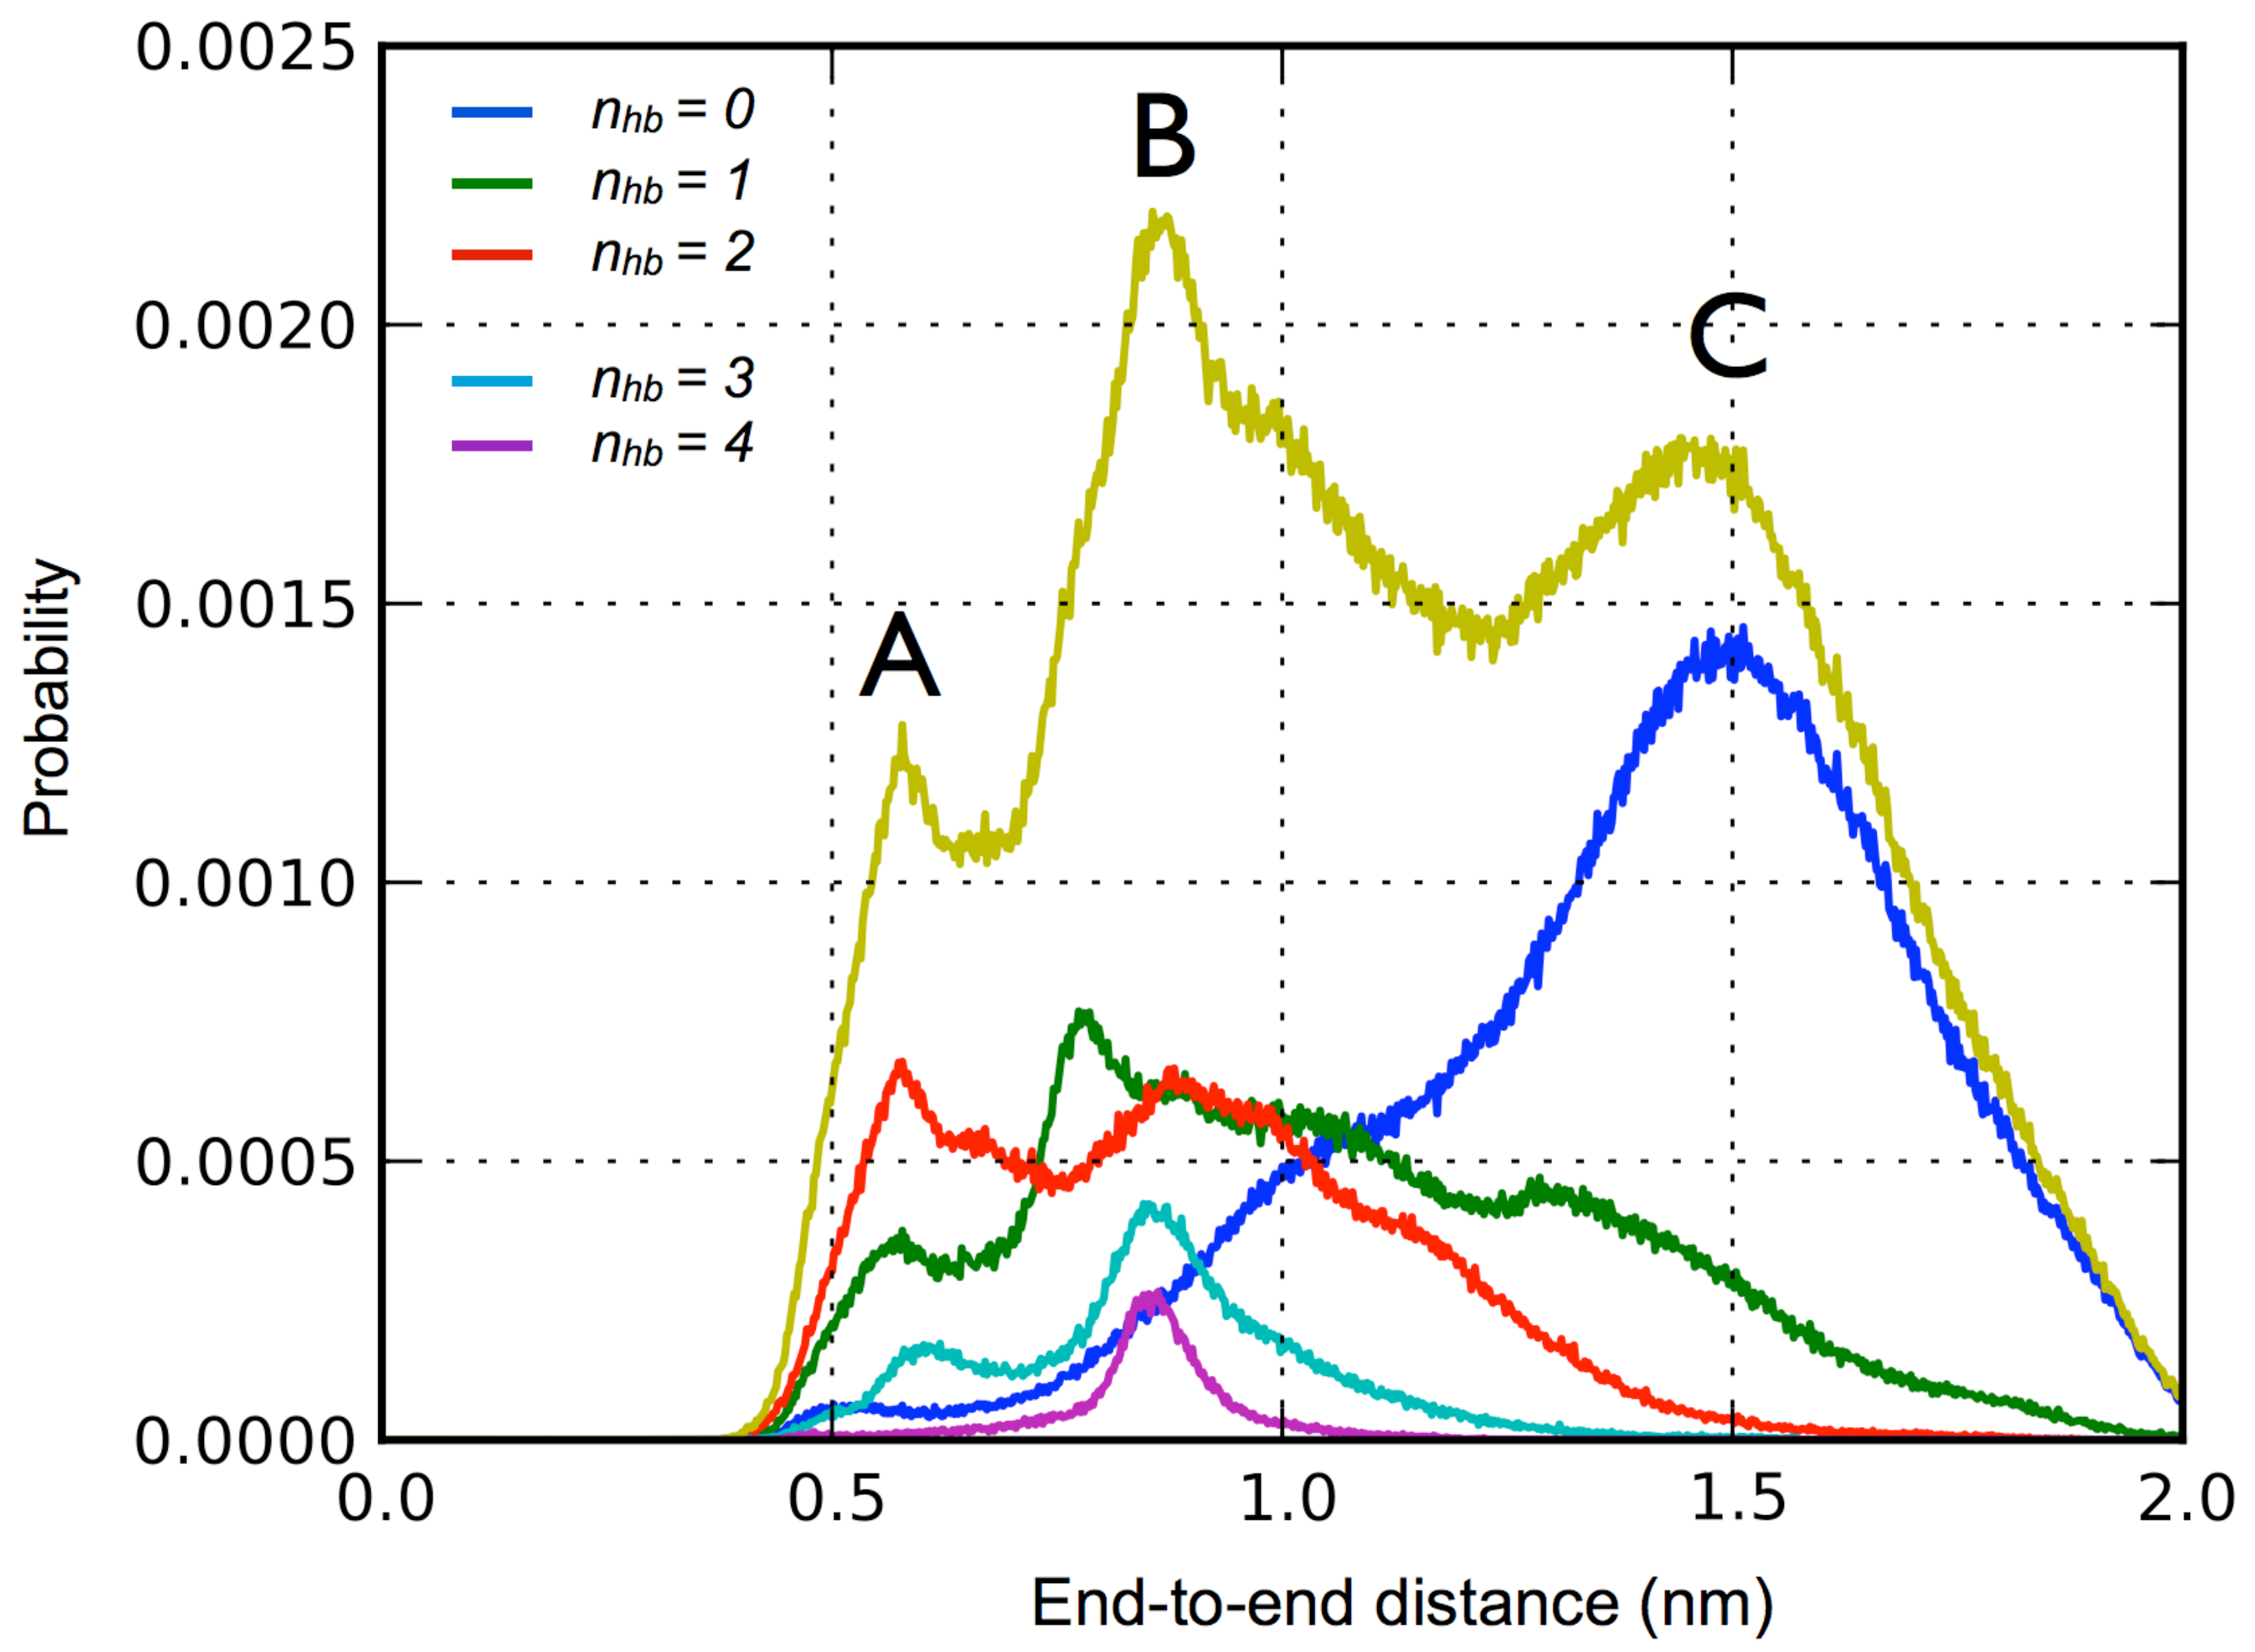
\includegraphics[width=14cm]{figures/appendixA/inos2_figures_SI_monomer_eed_by_hbonds.pdf}
\caption[The end-to-end distance distribution of monomeric A$\beta$(16-22) conformations separated by the number of intra-peptide hydrogen bonds, $n_{hb}$.]{The end-to-end distance distribution of monomeric A$\beta$(16-22) conformations separated by the number of intra-peptide hydrogen bonds, $n_{hb}$. The curve in yellow is the end-to-end distribution over all peptide conformations. The peaks at (A) 0.55 nm, (B) 0.9 nm, and (C) 1.4 nm generally correspond to peptide conformations with a $\beta$-bridge between residues Leu17 and Phe20, with 1 or more intermolecular hydrogen bonds, and with no intra-peptide hydrogen bonds, respectively.}
\label{fig:SI-monomersEedByHbonds}
\end{figure}

\begin{figure}[ht]
\centering
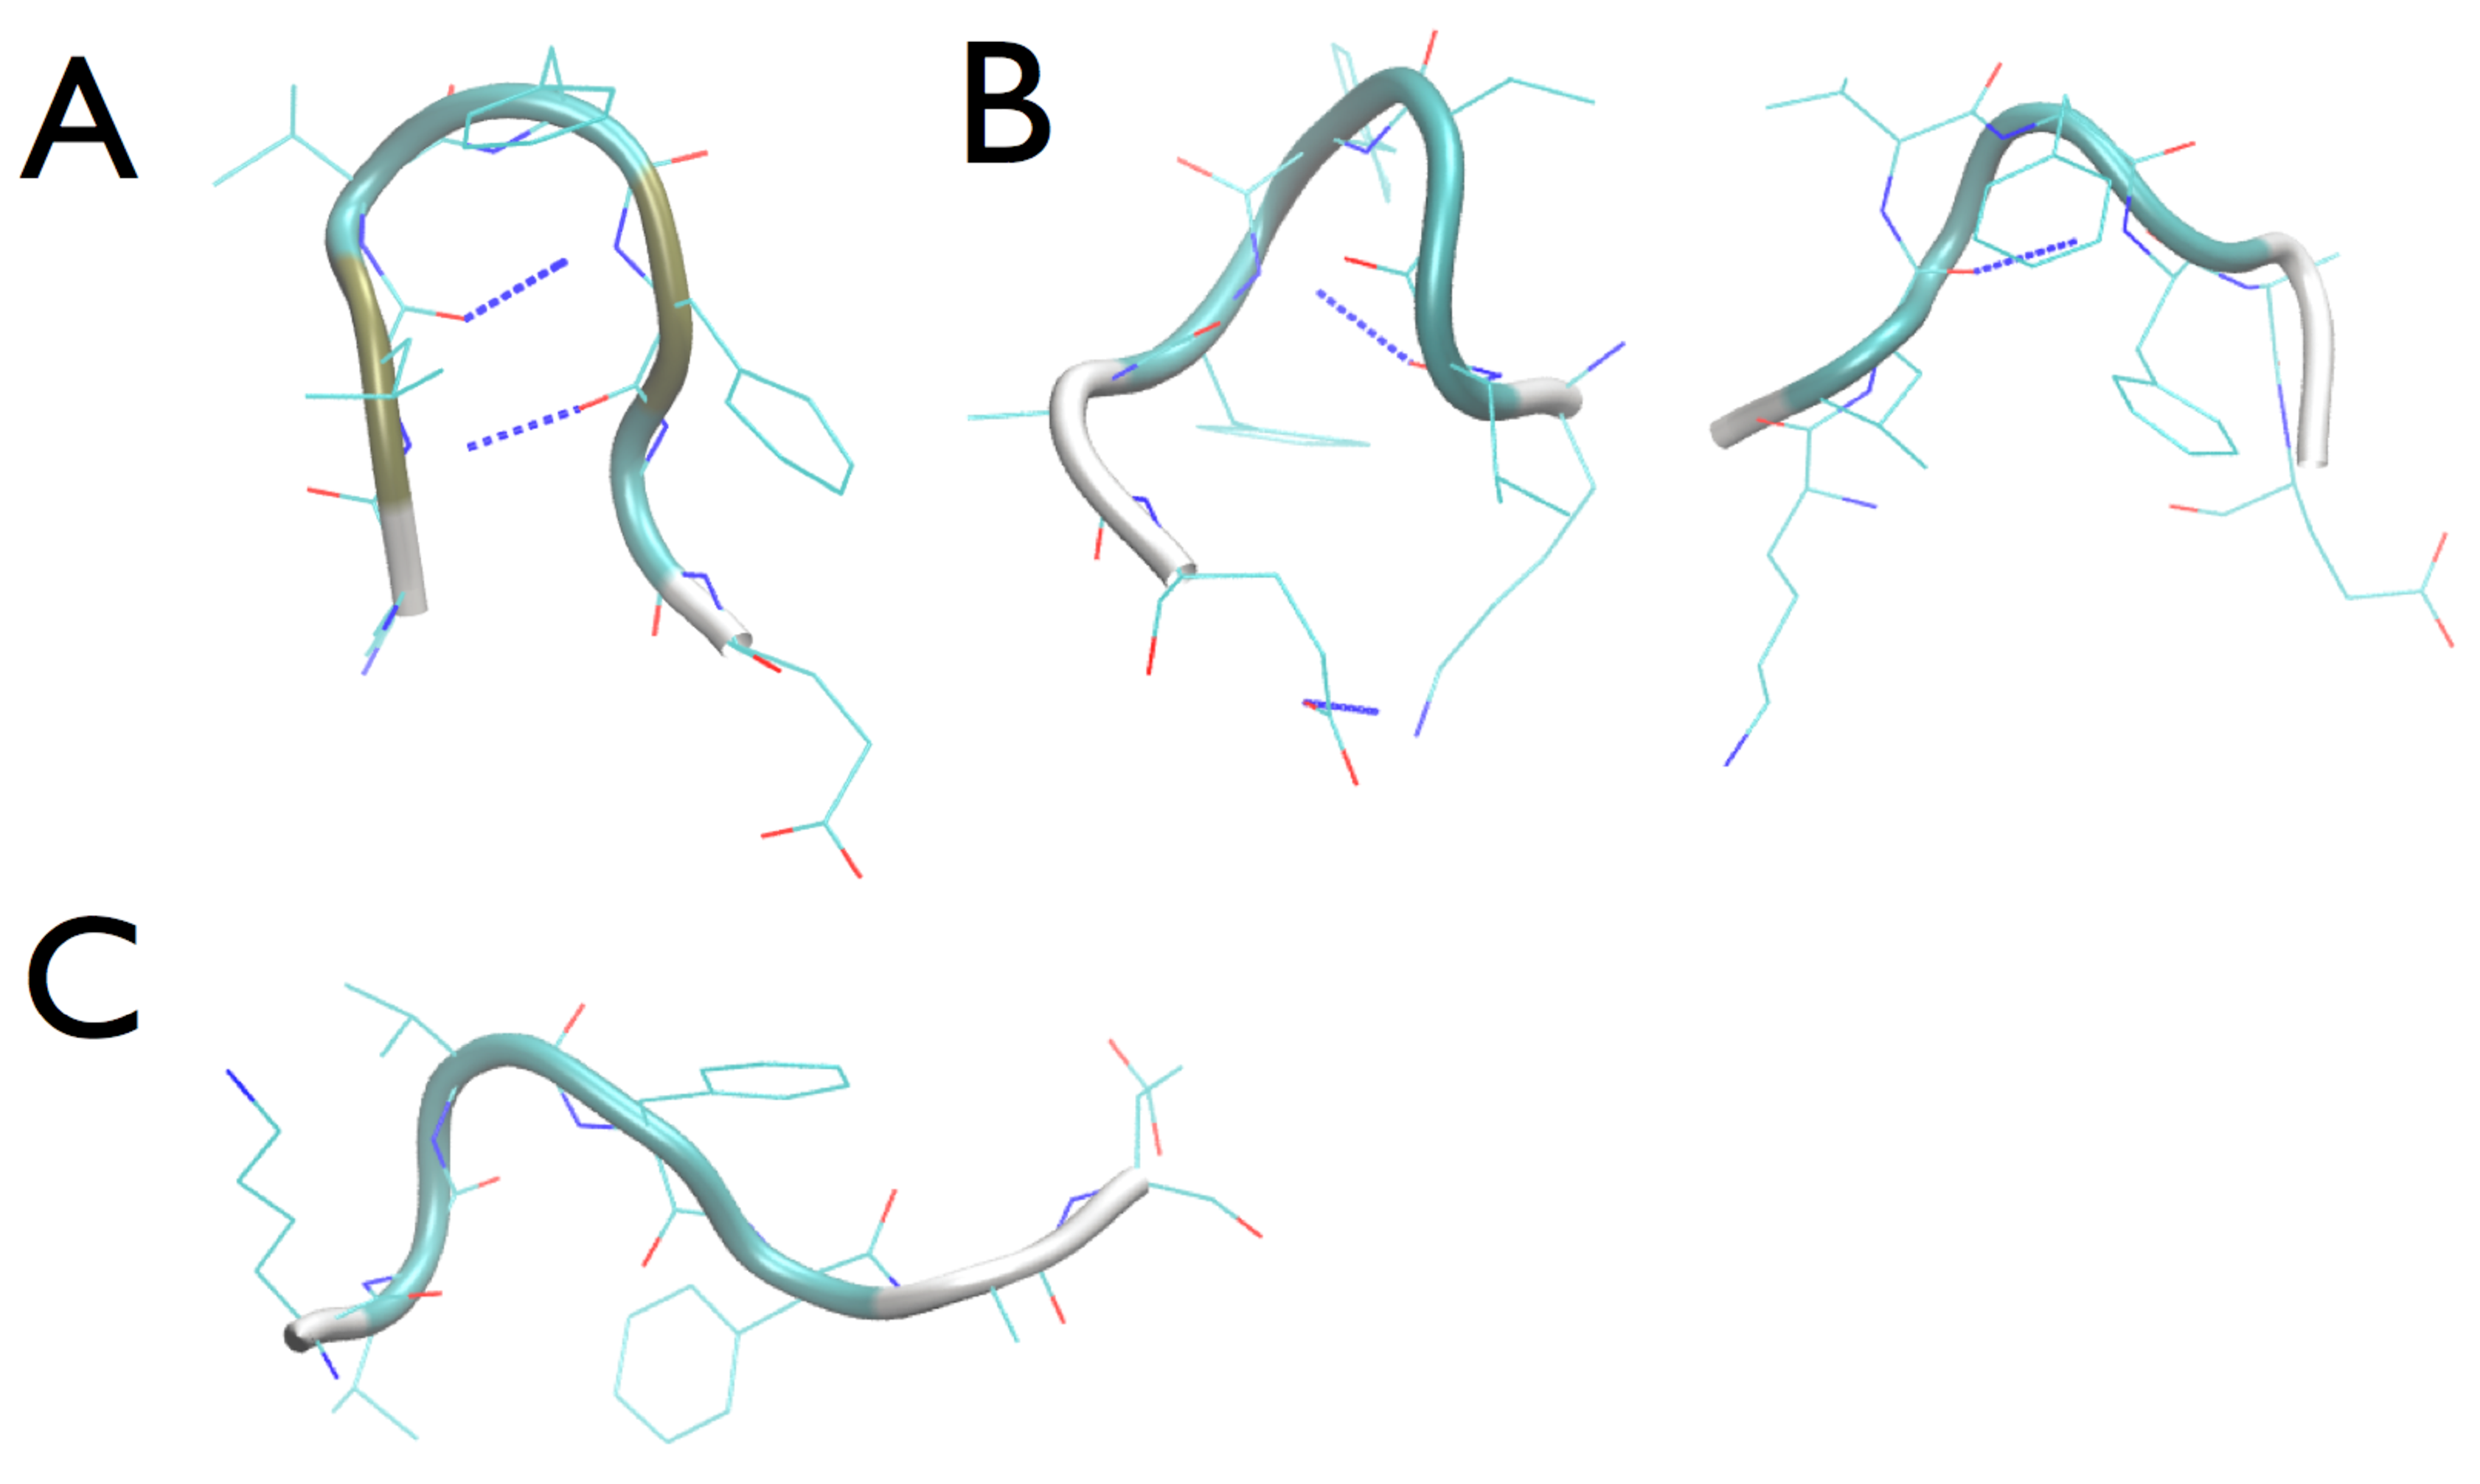
\includegraphics[width=14cm]{figures/appendixA/inos2_figures_SI_monomerConformations.pdf}
\caption[Snapshots of representative monomer conformations at each peak of the end-to-end distribution.]{Snapshots of representative monomer conformations at each peak of the end-to-end distribution. 
(A)  Compact conformations with end-to-end distances of $\sim$0.59 nm correspond to an ensemble of peptides with a $\beta$-bridge formed between Leu and Phe. (B) Representative conformations of the peak at 0.8-0.9 nm are predominantly peptides with a single hydrogen-bonded turn formed between residues Val and Phe20. Furthermore, the end-to-end distance of this peak also captures conformers with salt bridges, which account for the populations with $n_{hb}$ = 3 or $n_{hb}$ = 4. (C)  Extended peptide conformations have no intra-peptide hydrogen bonds, and have end-to-end distances corresponding to the peak in the distribution at $\sim$1.4 nm.}
\label{fig:SI-monomersConformations}
\end{figure}

\begin{table}[ht]
\centering
\begin{tabular}{|l|llll|}
\hline
\multicolumn{5}{|c|}{2:1 (inositol:peptide)} \\ 
\hline
& \emph{scyllo} & \emph{chiro} & $s_{\overline{x}, \emph{scyllo}}$ & $s_{\overline{x}, \emph{chiro}}$ \\ 
\hline
Nonpolar & 37 & 45 & 2 & 2 \\ 
Nonpolar and Hbonds & 35 & 34 & 1 & 2 \\ 
Hbonds & 28 & 21 & 2 & 1 \\
\hline
\hline
\multicolumn{5}{|c|}{15:1} \\ 
\hline
 & \emph{scyllo} & \emph{chiro} & $s_{\overline{x}, \emph{scyllo}}$ & $s_{\overline{x}, \emph{chiro}}$ \\ 
\hline
Nonpolar & 36 & 45 & 1 & 1 \\
Nonpolar and Hbonds & 36 & 34 & 1 & 1 \\ 
Hbonds & 28 & 21 & 1 & 1 \\
\hline
\end{tabular}
\caption{Fraction of inositol molecules (in \%) bound to nonpolar and polar groups of the monomer.}    
\label{tbl:SI-monomersBindingMode}
\end{table}

\begin{figure}[ht]
\centering
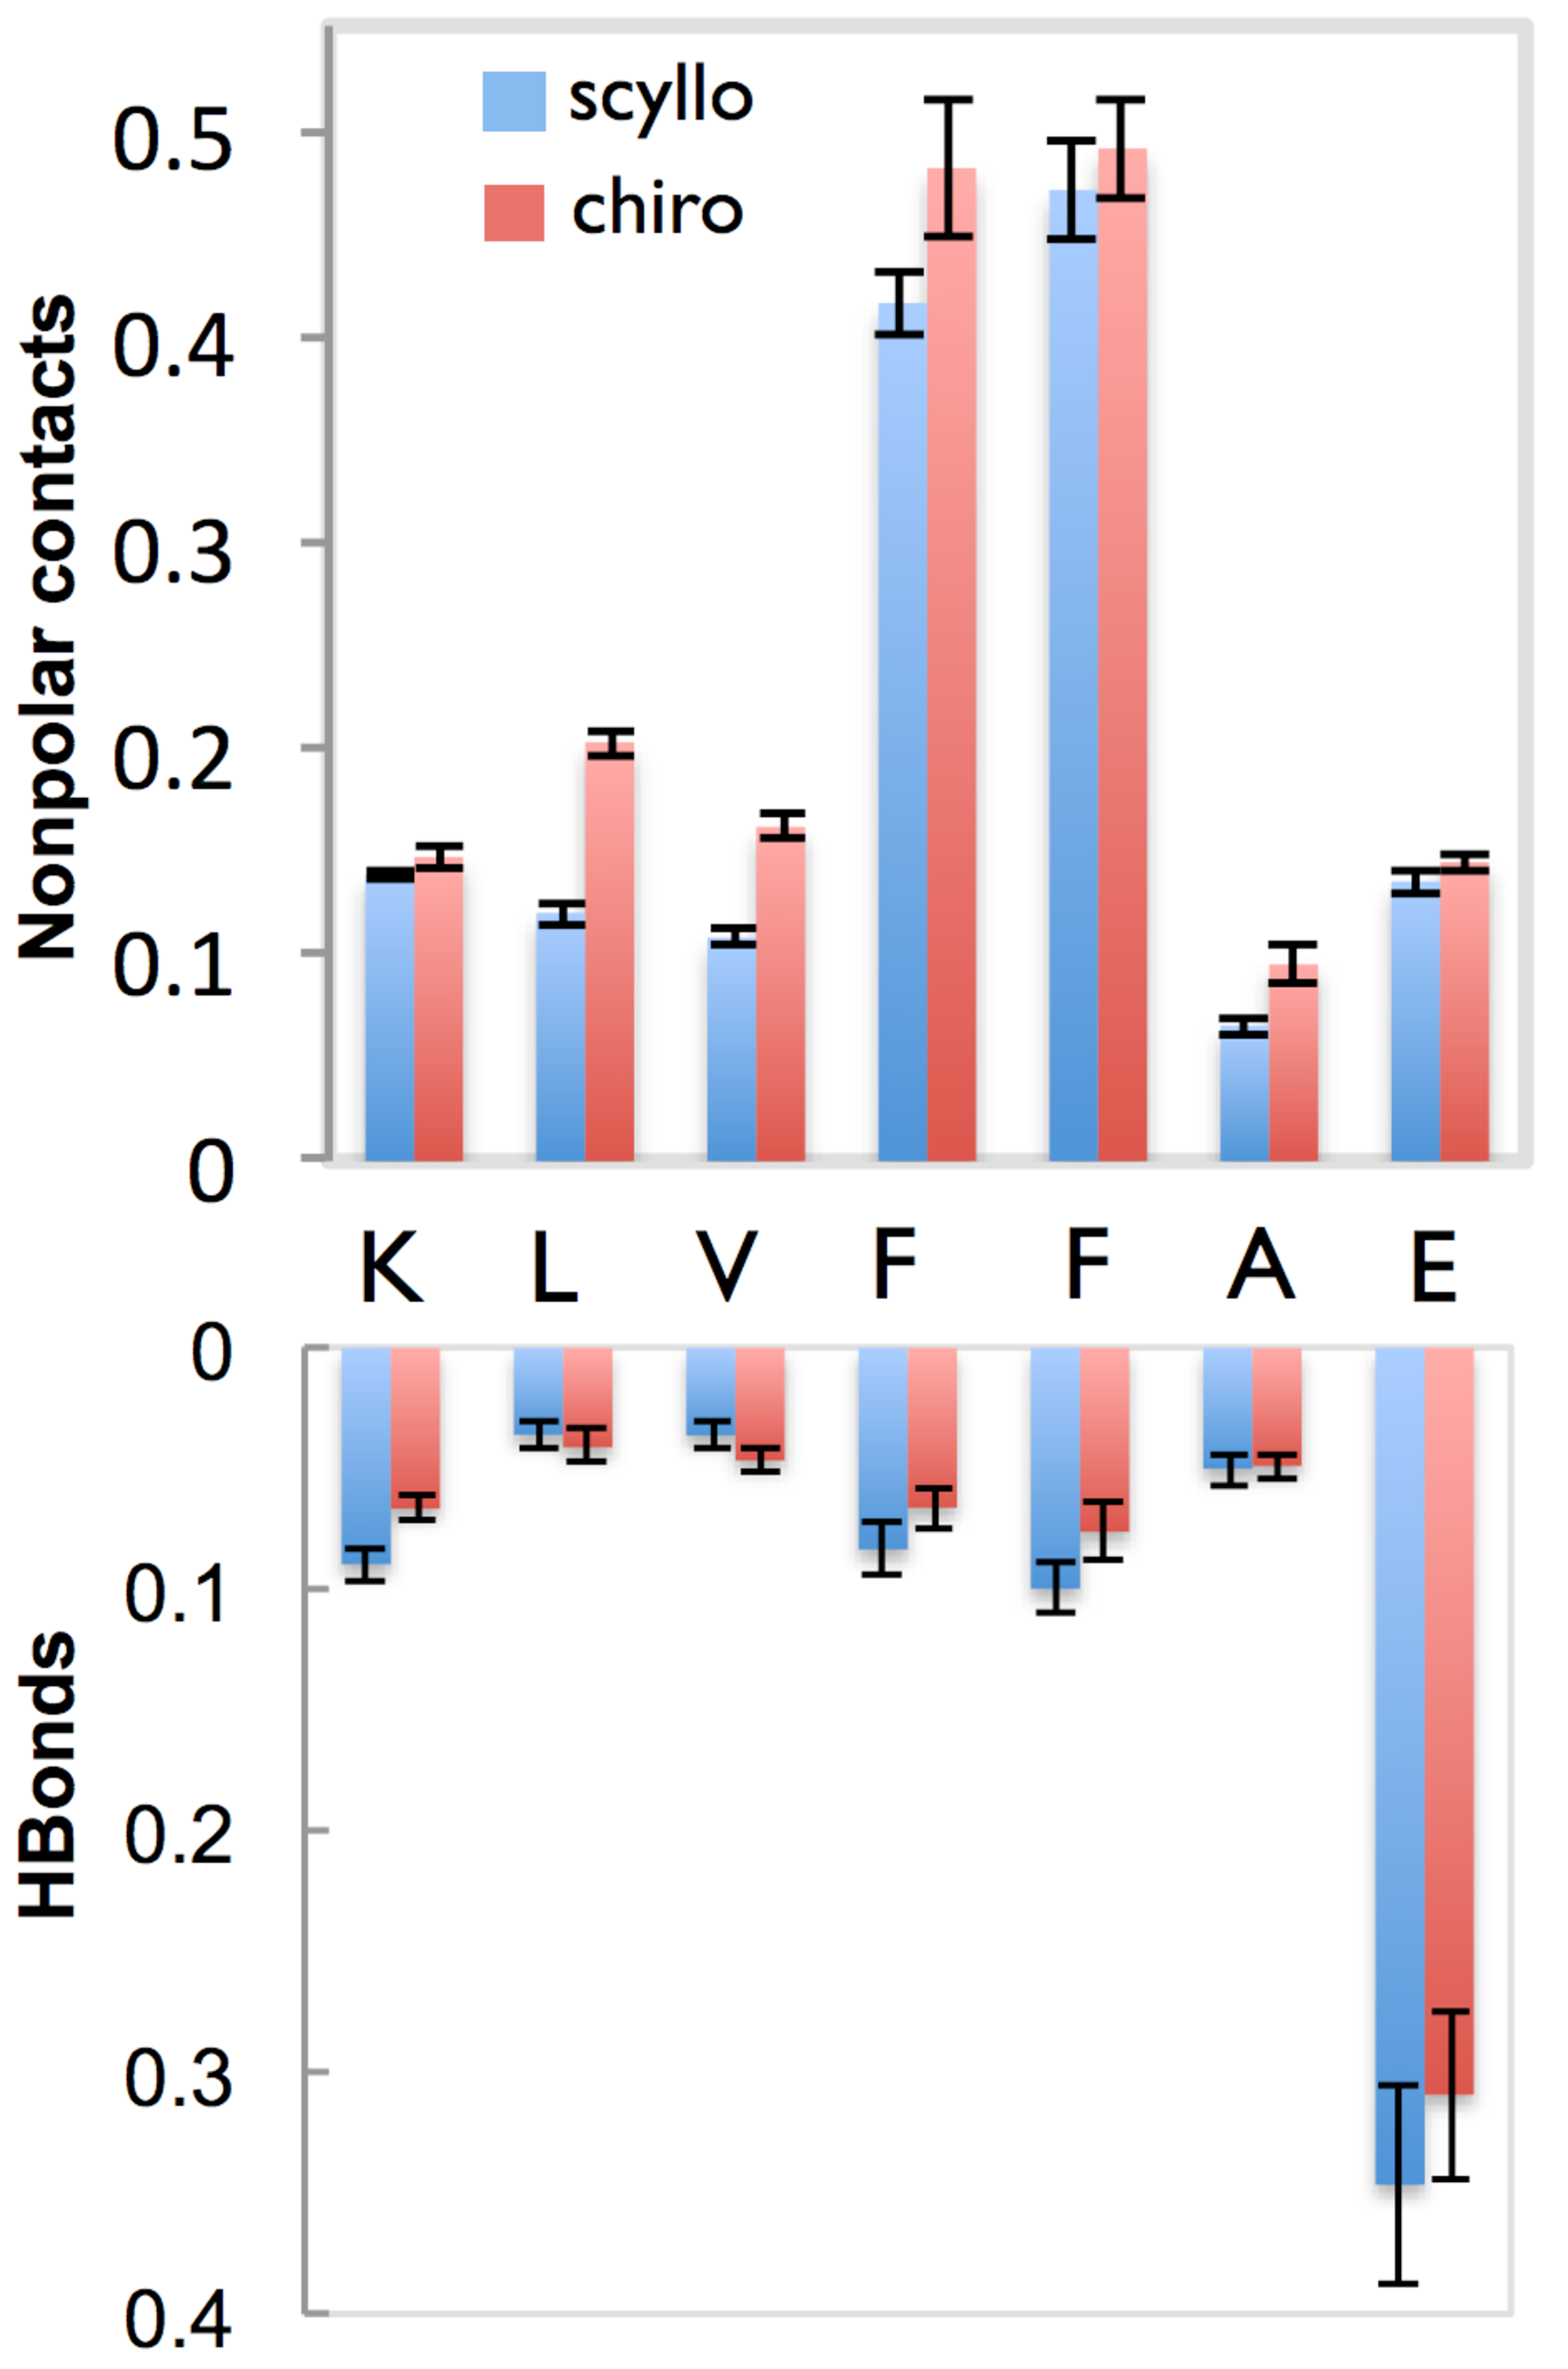
\includegraphics[width=8.21cm]{figures/appendixA/inos2_figures_SI_monomerBinding.pdf}
\caption[Time-averaged number of hydrogen bonds and nonpolar made by inositol to each residue of the monomer at an inositol:peptide molar ratio of 2:1.]{Time-averaged number of hydrogen bonds (top), and nonpolar (bottom) made by inositol to each residue of the monomer at an inositol:peptide molar ratio of 2:1.}
\label{fig:SI-monomersBinding}
\end{figure}

\clearpage
\newpage

\section{Disordered Oligomer}

\begin{table}[ht]
\centering 
\begin{tabular}{|l|llll|}
\hline
\multicolumn{5}{|c|}{2:4 (inositol:peptide)} \\ \hline
& \emph{scyllo} & \emph{chiro} & $s_{\overline{x}, \emph{scyllo}}$ & $s_{\overline{x}, \emph{chiro}}$ \\
\hline
Nonpolar & 36 & 51 & 6 & 4 \\ 
Nonpolar and Hbonds & 20 & 23 & 3 & 2 \\ 
Hbonds & 44 & 26 & 5 & 3 \\
\hline
\hline
\multicolumn{5}{|c|}{15:4} \\
\hline
& \emph{scyllo} & \emph{chiro} & $s_{\overline{x}, \emph{scyllo}}$ & $s_{\overline{x}, \emph{chiro}}$ \\
\hline
Nonpolar & 26 & 36 & 2 & 5 \\ 
Nonpolar and Hbonds & 51 & 48 & 2 & 4 \\ 
Hbonds & 23 & 16 & 3 & 2 \\
\hline
\hline
\multicolumn{5}{|c|}{45:4} \\
\hline
& \emph{scyllo} & \emph{chiro} & $s_{\overline{x}, \emph{scyllo}}$ & $s_{\overline{x}, \emph{chiro}}$ \\
\hline
Nonpolar & 30 & 36 & 2 & 3 \\ 
Nonpolar and Hbonds & 48 & 47 & 3 & 3 \\ 
Hbonds & 23 & 17 & 3 & 2 \\
\hline
\end{tabular}
\caption{Fraction of inositol molecules (in \%) bound to nonpolar and polar groups of the disordered oligomer.}    
\label{tbl:SI-disorderedBindingMode}
\end{table}


\begin{figure}[ht]
\centering
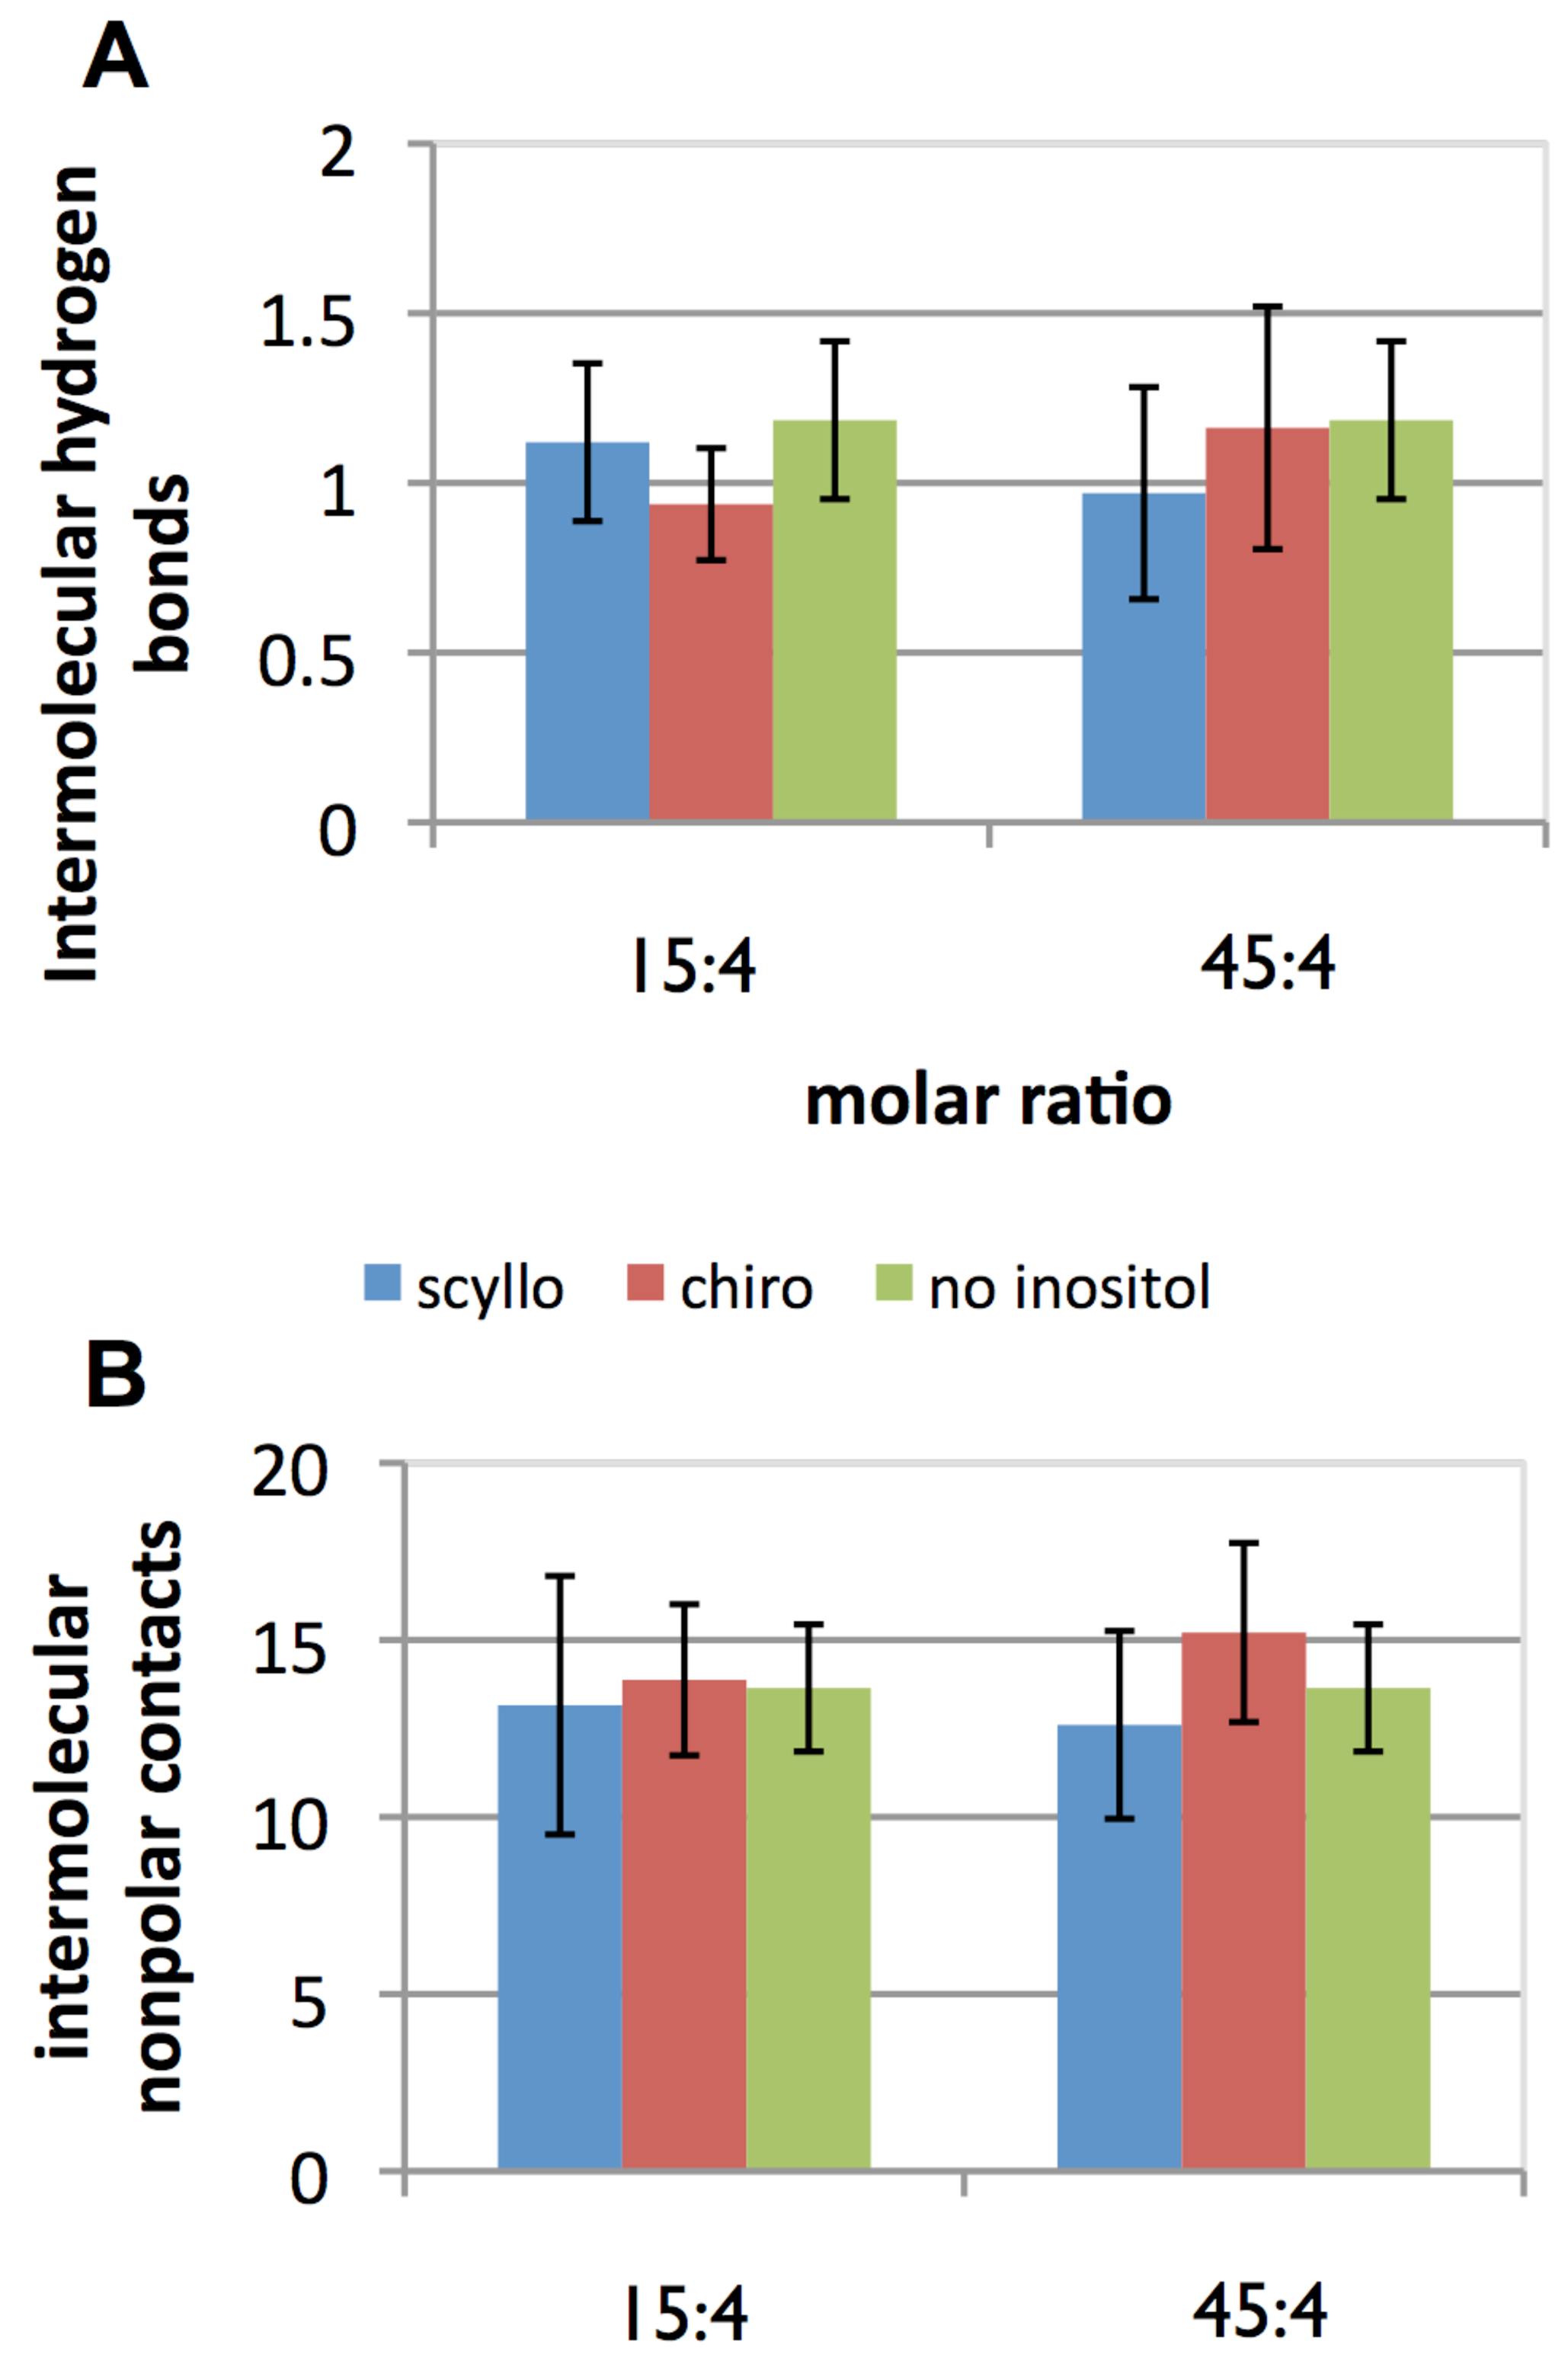
\includegraphics[width=8.25cm]{figures/appendixA/inos2_figures_SI_disorderedNumContacts.pdf}
\caption[The equilibrium number of intermolecular contacts per peptide in the disordered oligomer]{The equilibrium number of intermolecular (A) hydrogen bonding, and (B) nonpolar contacts per peptide in the disordered oligomer.}
\label{fig:SI-disorderedNumContacts}
\end{figure}

\begin{figure}[ht]
\centering
% Needs to be decreased in height
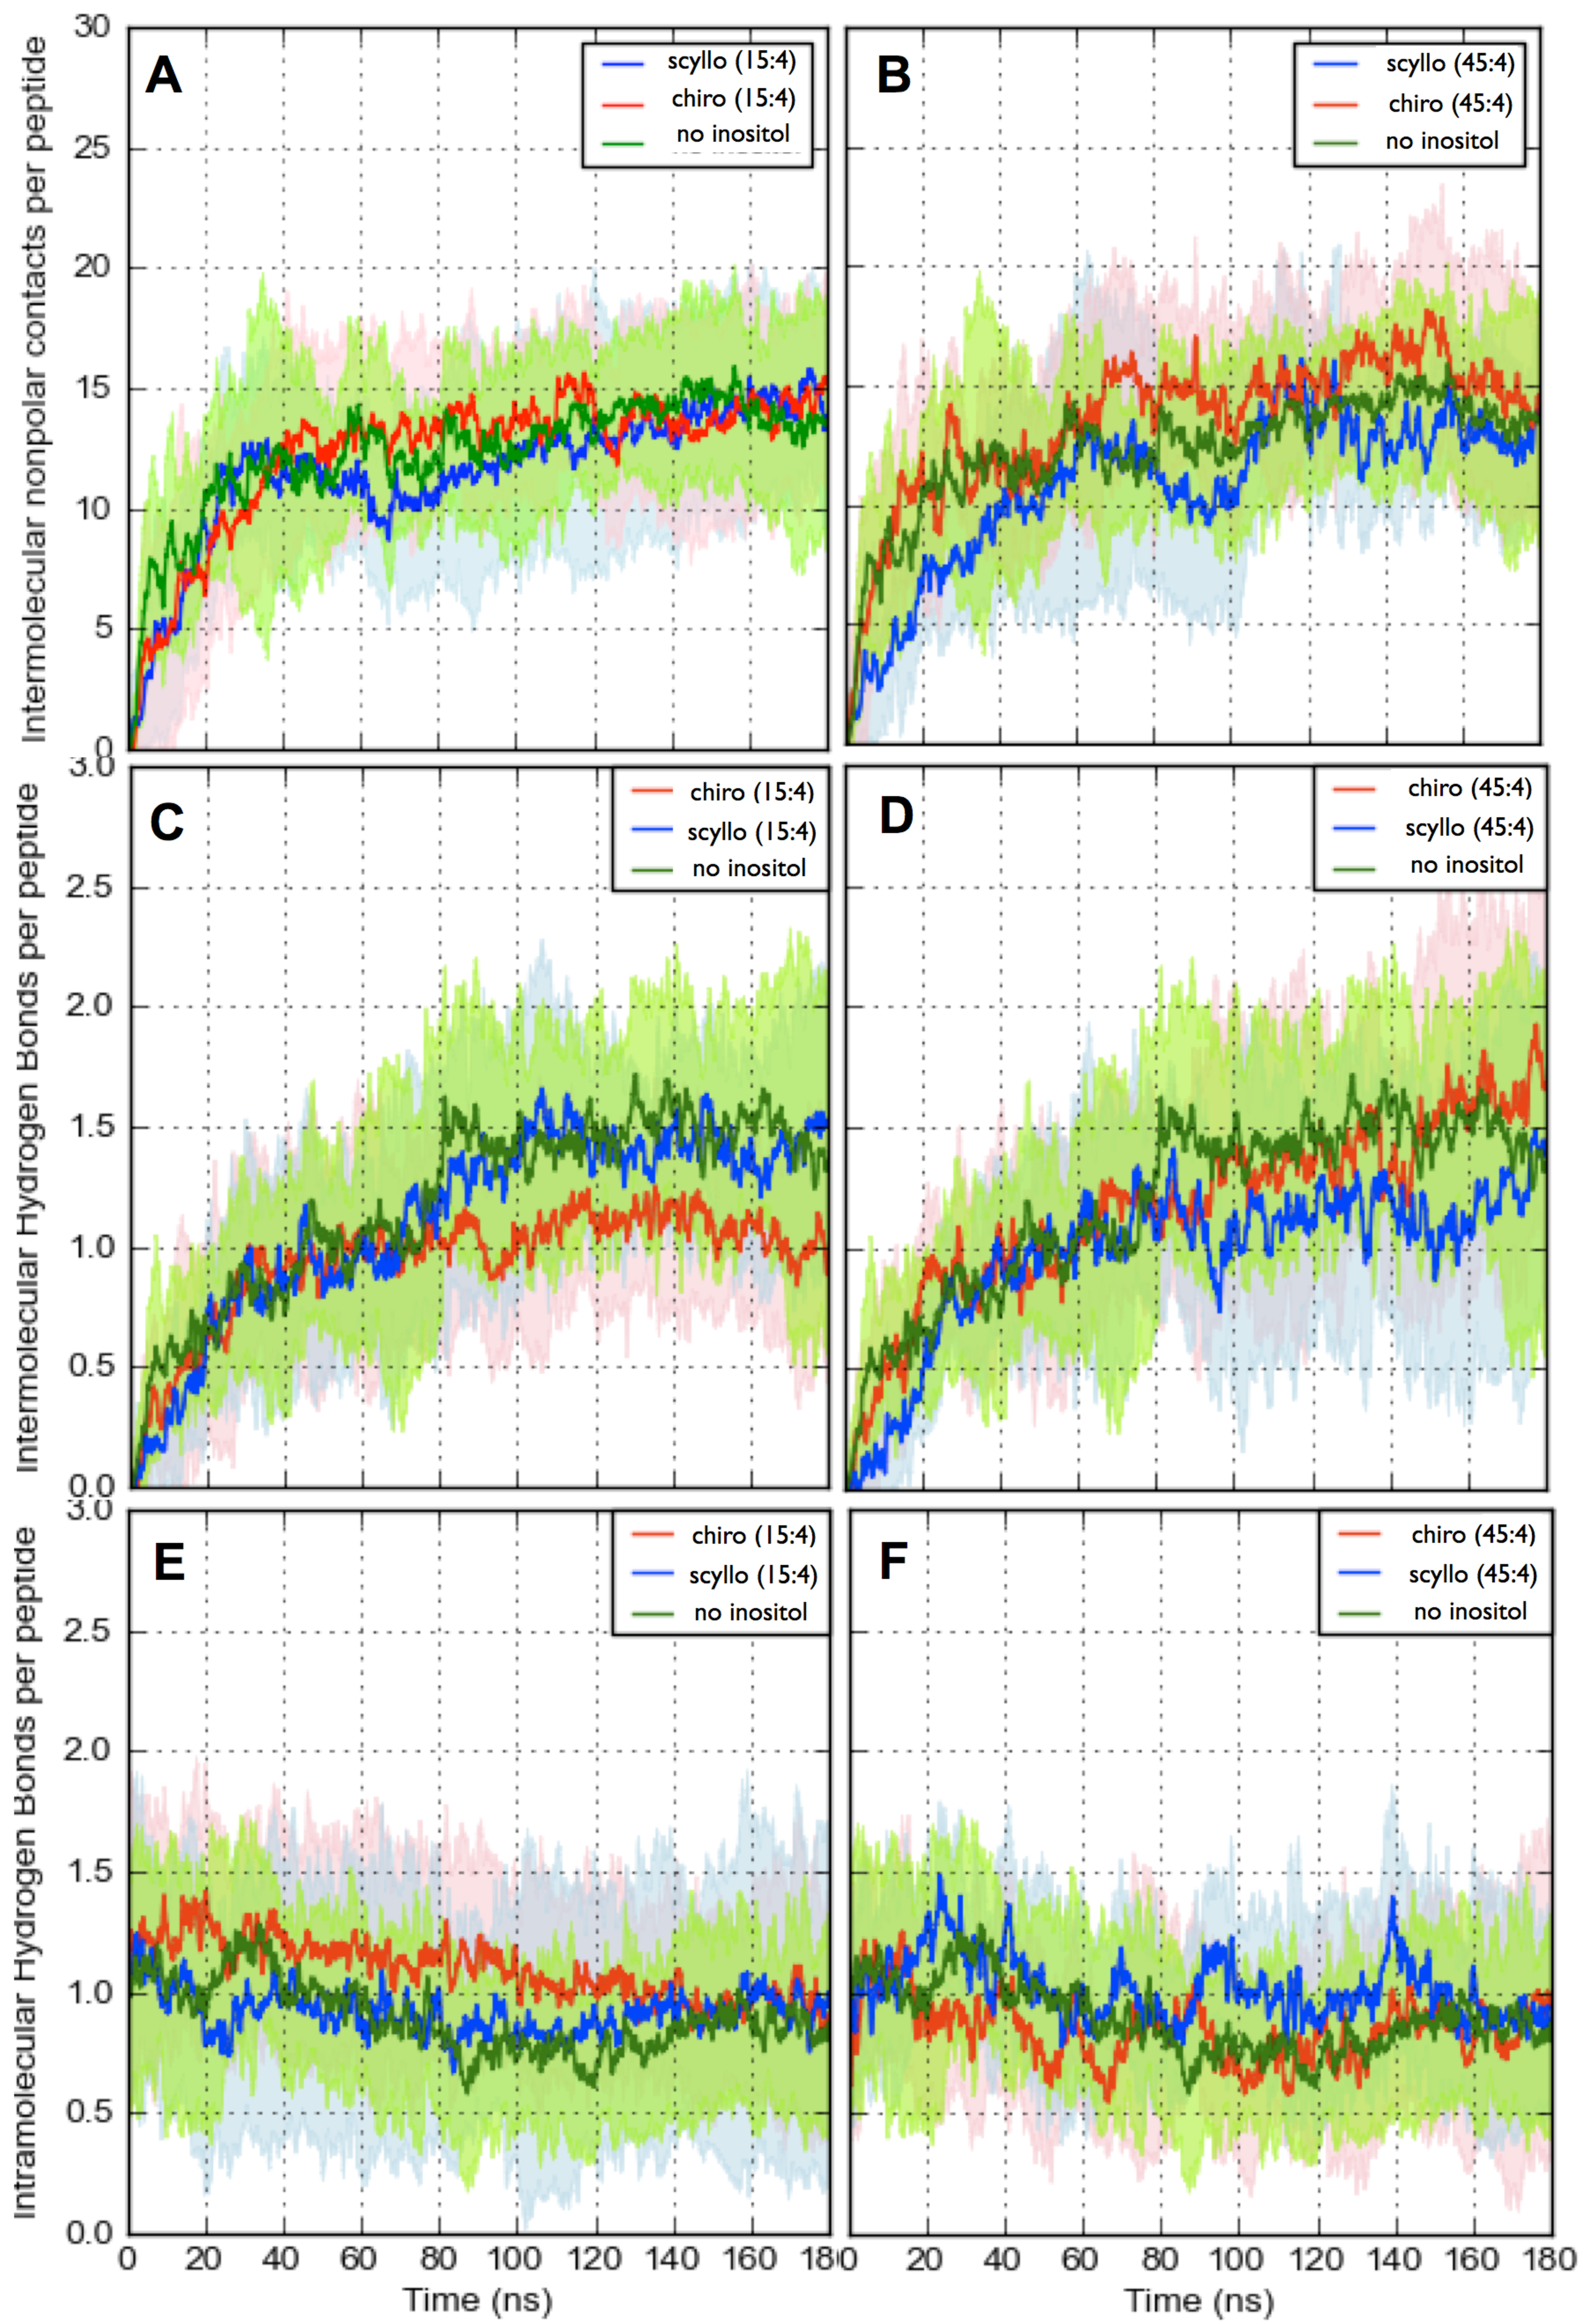
\includegraphics[width=14cm]{figures/appendixA/inos2_figures_SI_disorderedContactTS.pdf}
\caption[Effect of inositol on the aggregation of A$\beta$(16-22)]{Effect of inositol on the aggregation of A$\beta$(16-22). Data for inositol:peptide molar ratios 15:4 and 45:4 are shown on the left and right panel, respectively. (A)-(B) Time evolution of the peptide-peptide intermolecular nonpolar contacts per peptide. (C)-(D) Intermolecular peptide-peptide hydrogen bonds per peptide, and (E)-(F) intramolecular peptide-peptide hydrogen bonds per peptide. The time series were smoothed using a running average with a window of length 500 ps.}
\label{fig:SI-disorderedContactsTS}
\end{figure}

\begin{figure}[ht]
\centering
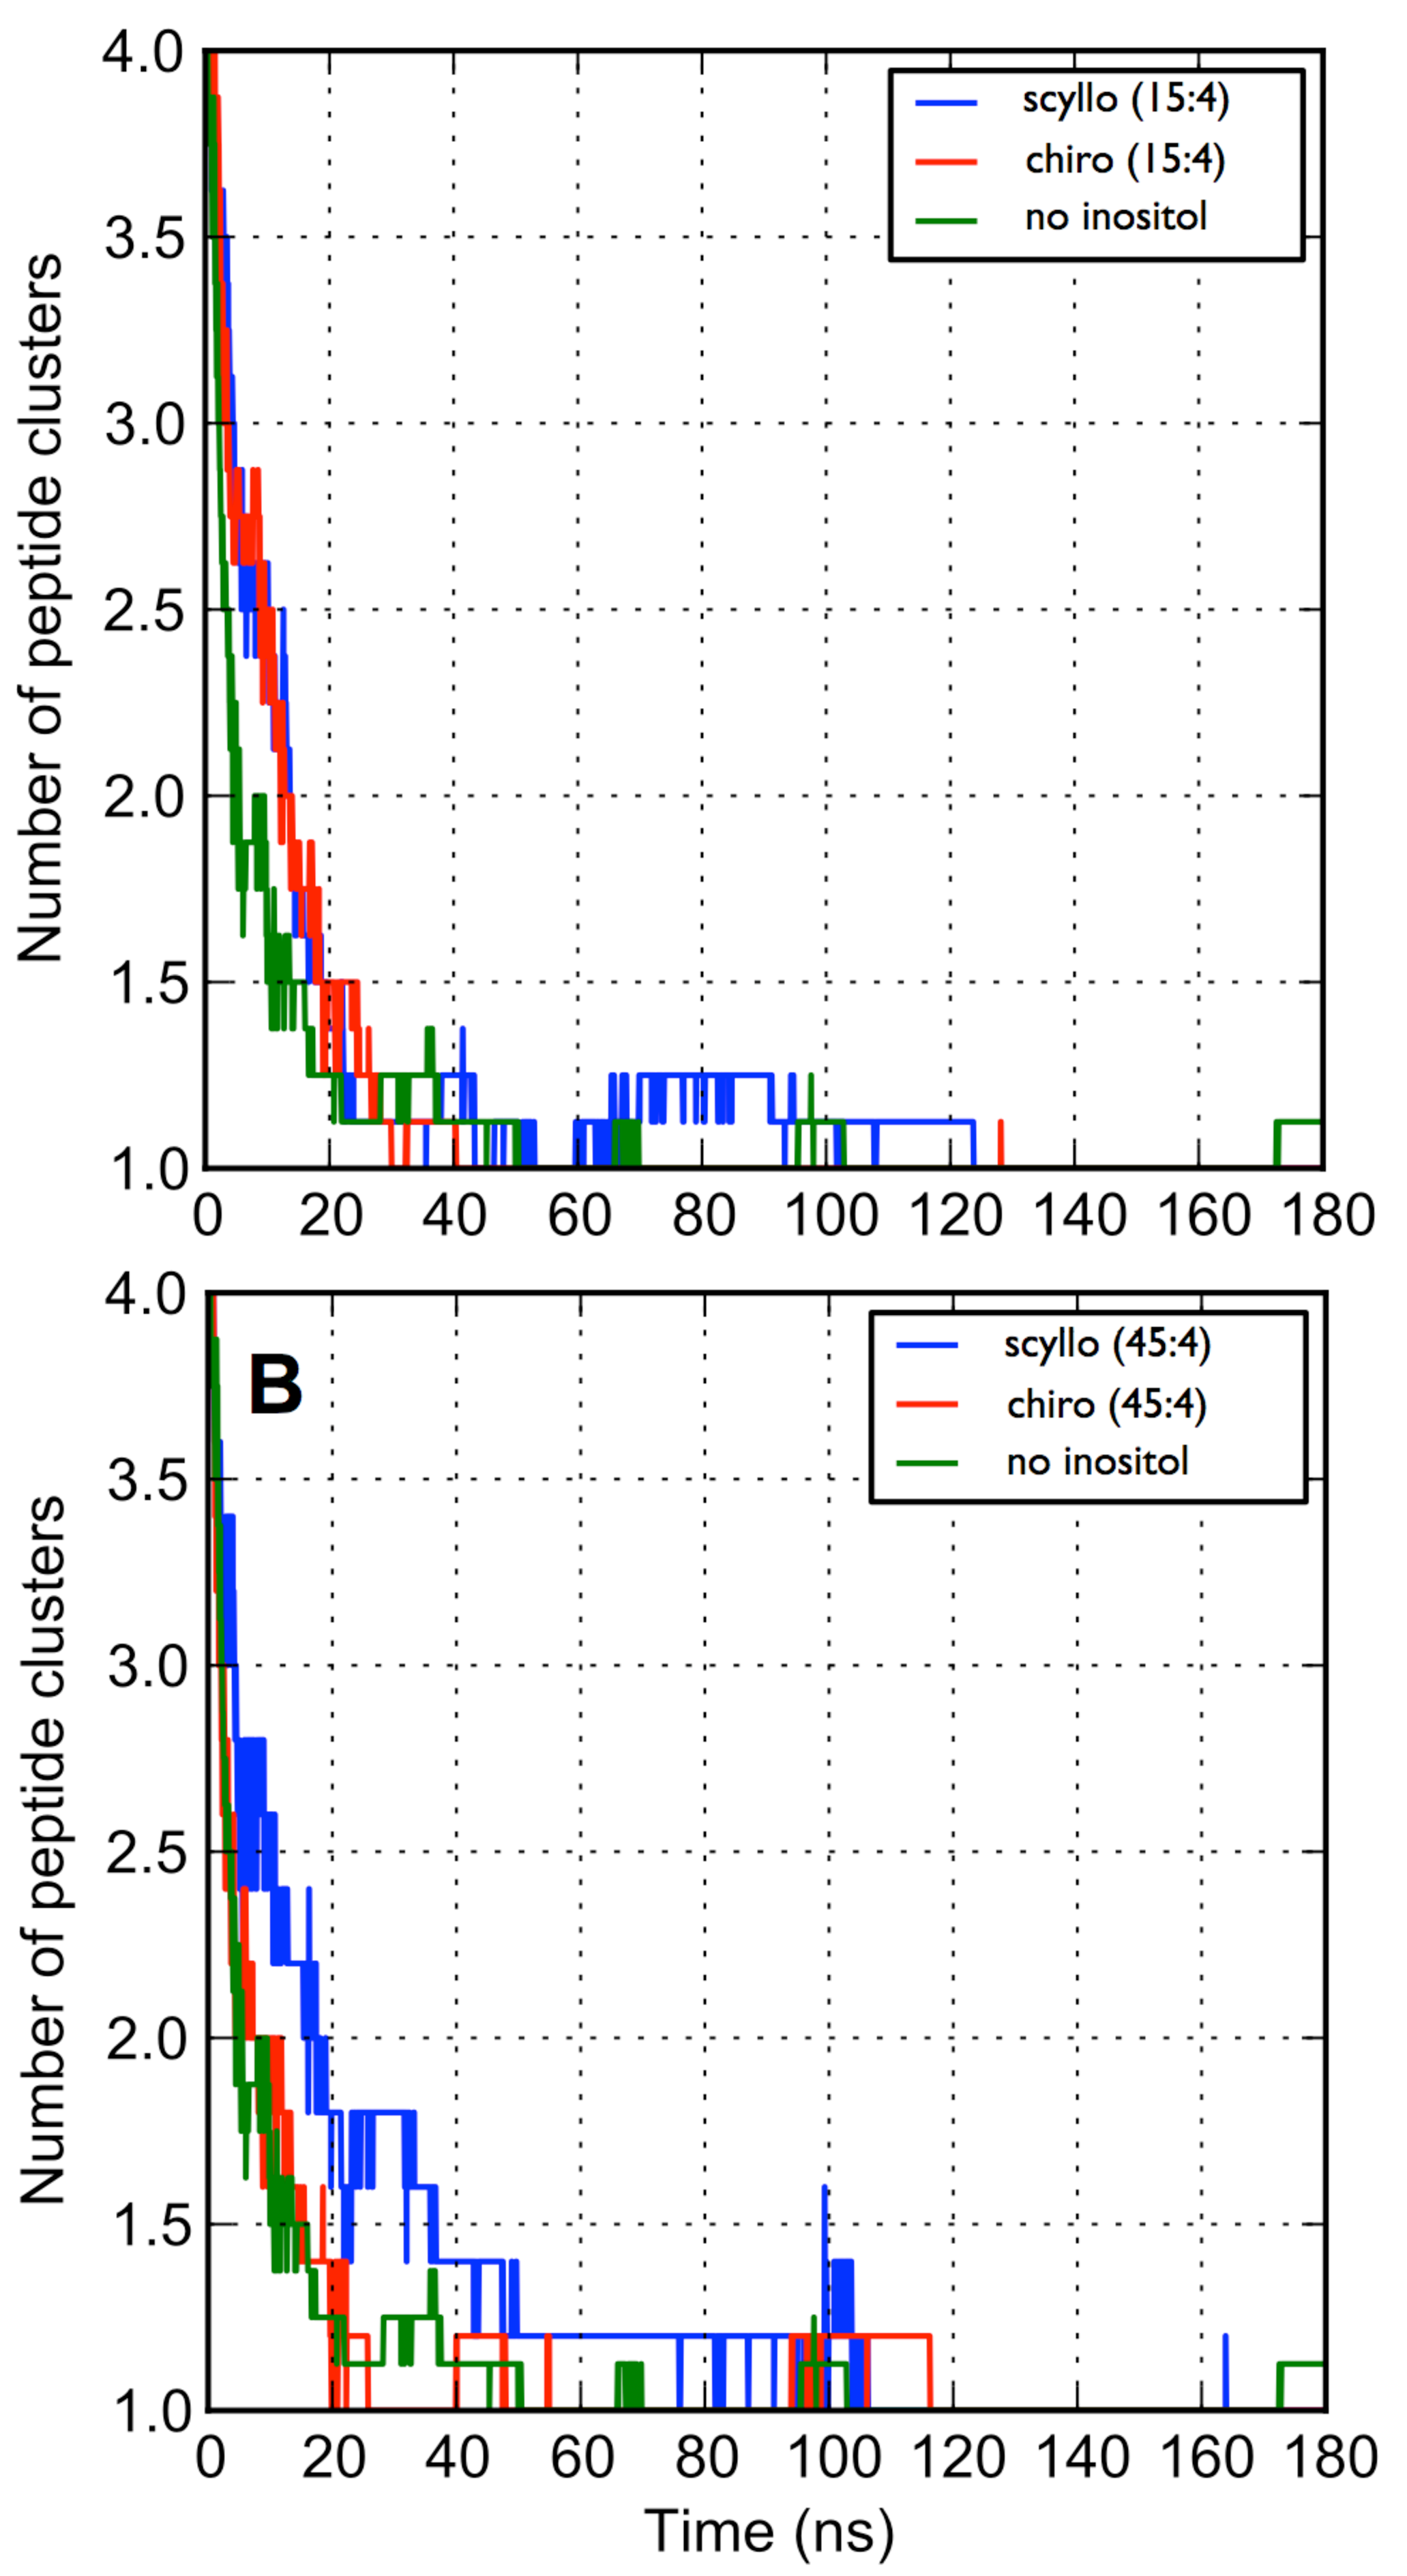
\includegraphics[width=8.25cm]{figures/appendixA/inos2_figures_SI_disorderedCluster.pdf}
\caption[Time-evolution of peptide self-aggregation to form the disordered oligomer]{Time-evolution of peptide self-aggregation to form the disordered oligomer at inositol:peptide molar ratios of (A) 15:4 and (B) 45:4.}
\label{fig:SI-disorderedCluster}
\end{figure}

\begin{figure}[ht]
\centering
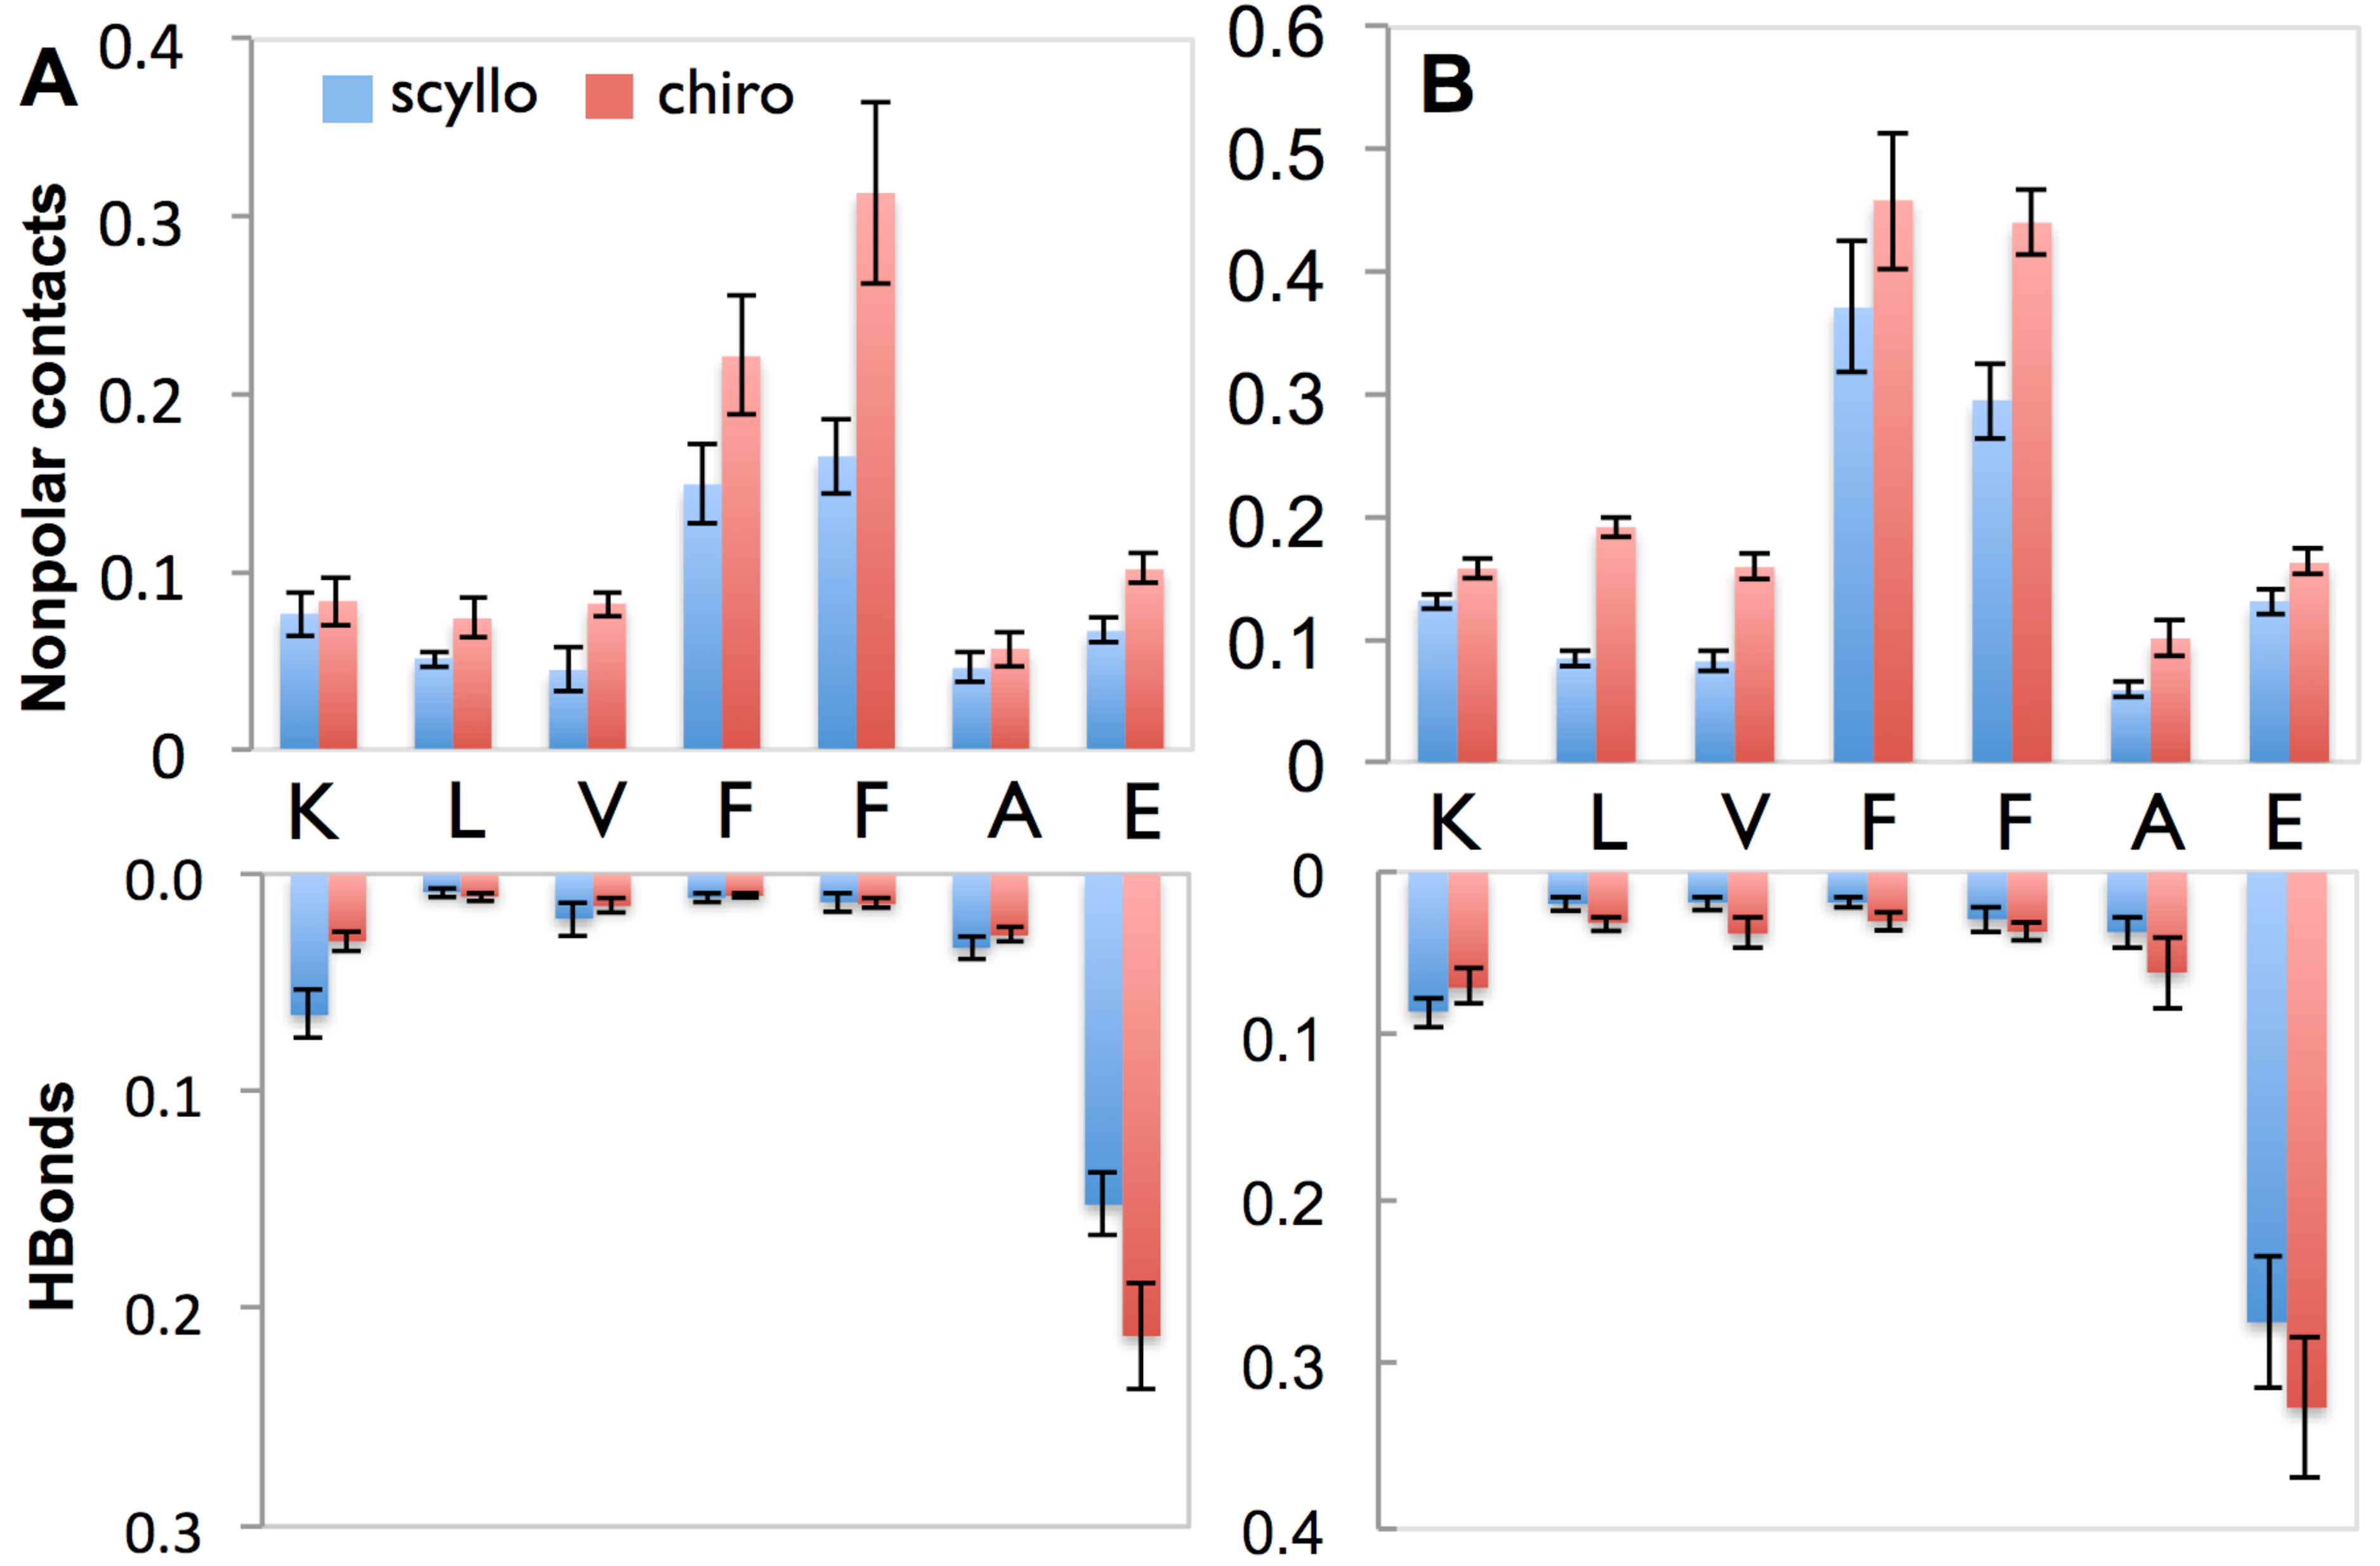
\includegraphics[width=14cm]{figures/appendixA/inos2_figures_SI_disorderedBinding_revised.pdf}
\caption[Time-averaged number of hydrogen bonds and nonpolar made by inositol to each residue of the disordered oligomer]{Time-averaged number of hydrogen bonds (top), and nonpolar (bottom) made by inositol to each residue of the disordered oligomer at an inositol:peptide molar ratios of (A) 2:4 and (B) 15:4.}
\label{fig:SI-disorderedBinding}
\end{figure}

\clearpage
\newpage

\section{$\beta$-oligomers}

\begin{table}[ht]
\centering
\begin{tabular}{|lllll|}
\hline
\multicolumn{5}{|c|}{4:16 (inositol:peptide), 37 mM (effective concentration)} \\
\hline
& \emph{scyllo} & \emph{chiro} & $s_{\overline{x}, \emph{scyllo}}$ & $s_{\overline{x}, \emph{chiro}}$ \\
\hline
Nonpolar & 23 & 33 & 1 & 2 \\
Nonpolar and Hbonds & 52 & 48 & 1 & 2 \\
Hbonds & 25 & 19 & 1 & 2 \\
\hline
\hline
\multicolumn{5}{|c|}{64:16, 63 mM} \\
\hline
& \emph{scyllo} & \emph{chiro} & $s_{\overline{x}, \emph{scyllo}}$ & $s_{\overline{x}, \emph{chiro}}$ \\ 
\hline
Nonpolar & 19 & 29 & 1 & 1 \\
Nonpolar and Hbonds & 58 & 56 & 1 & 1\\
Hbonds & 23 & 15 & 1 & 1 \\
\hline
\hline
\multicolumn{5}{|c|}{64:16, 200 mM} \\
\hline
& \emph{scyllo} & \emph{chiro} & $s_{\overline{x}, \emph{scyllo}}$ & $s_{\overline{x}, \emph{chiro}}$ \\
\hline
Nonpolar & 19.7 & 30 & 0.4 & 1 \\
Nonpolar and Hbonds & 56.7 & 54 & 0.5 & 1 \\
Hbonds & 23.5 & 16 & 0.3 & 1 \\
\hline
\end{tabular}
\caption{Fraction of inositol molecules (in \%) bound to nonpolar and polar groups of the $\beta$-oligomer.}    
\label{tbl:SI-betaBindingMode}
\end{table}

\begin{figure}[ht]
\centering
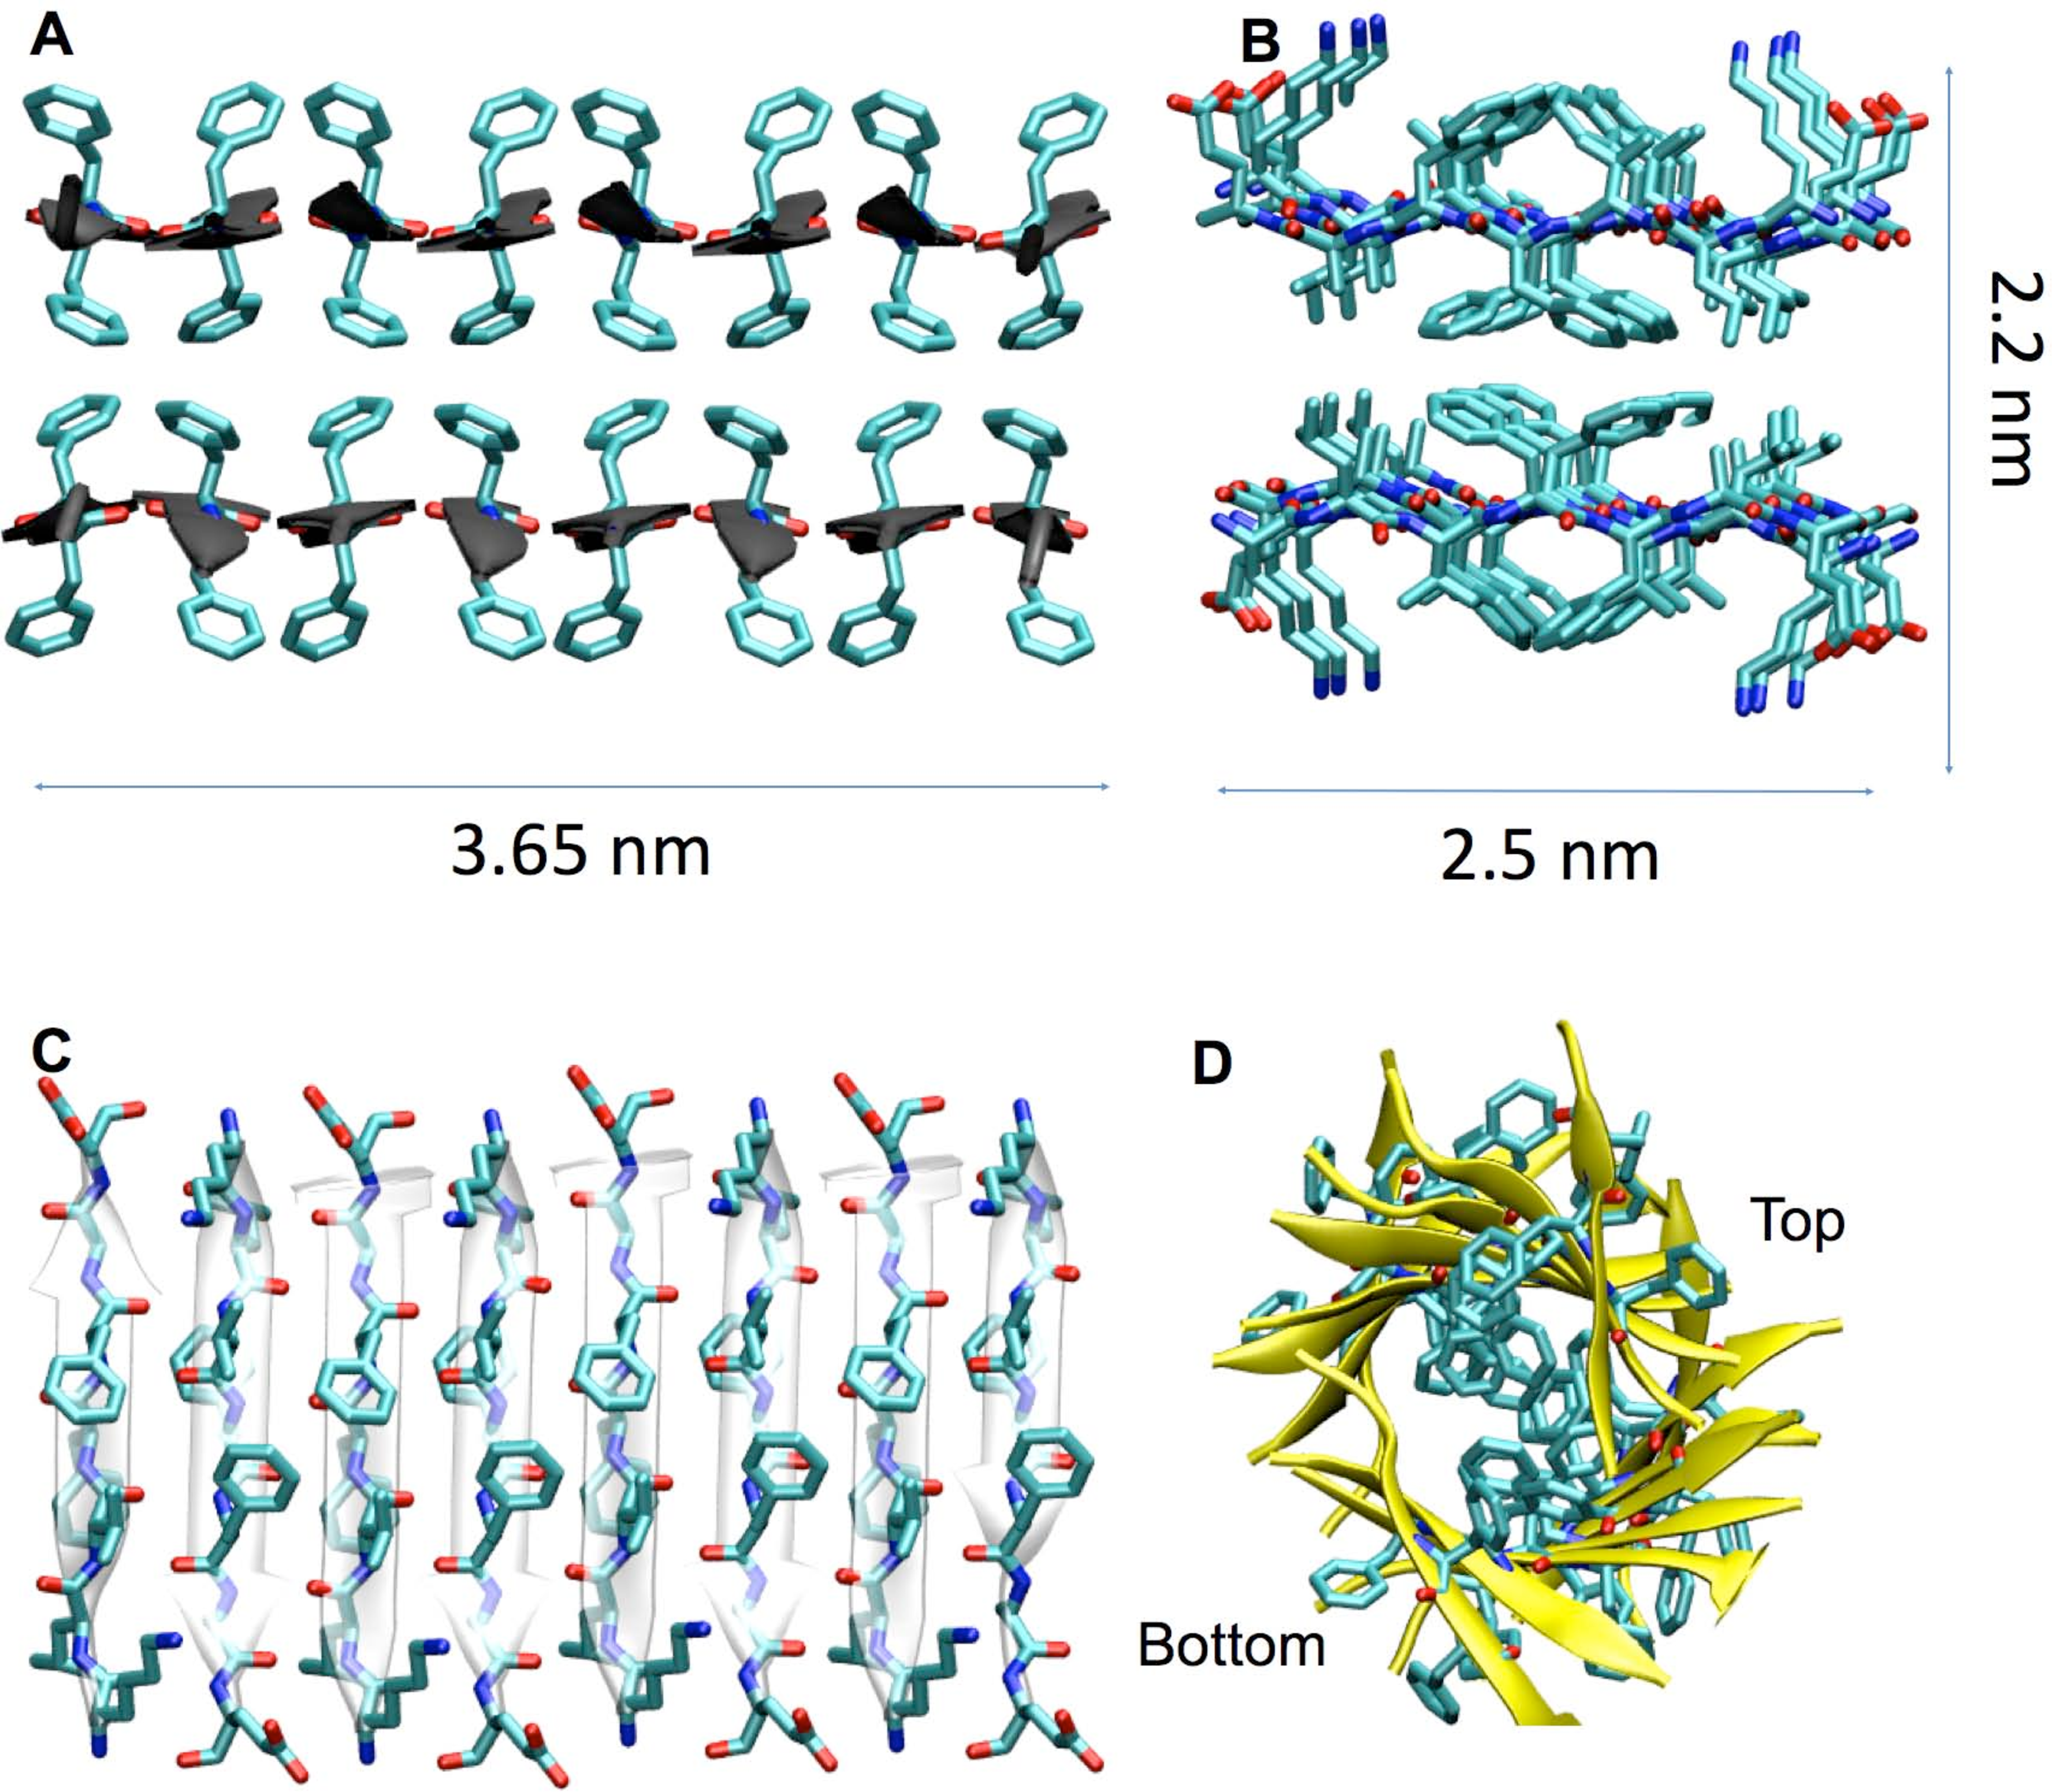
\includegraphics[width=15.15cm]{figures/appendixA/inos2_figures_SI_betaInitialModel.pdf}
\caption[Initial model of the $\beta$-oligomer]{Initial model of the $\beta$-oligomer. (A) Side view; (B) down the fibril axis, and (C) looking down at the face of the sheet. The initial starting structure of the oligomer has dimensions of 2.2 nm x 2.5 nm x 3.65 nm. (D) Snapshot of the $\beta$-oligomer from a simulation without inositol ($t=80$ ns).}
\label{fig:SI-betaInitialModel}
\end{figure}

\begin{figure}[ht]
\centering
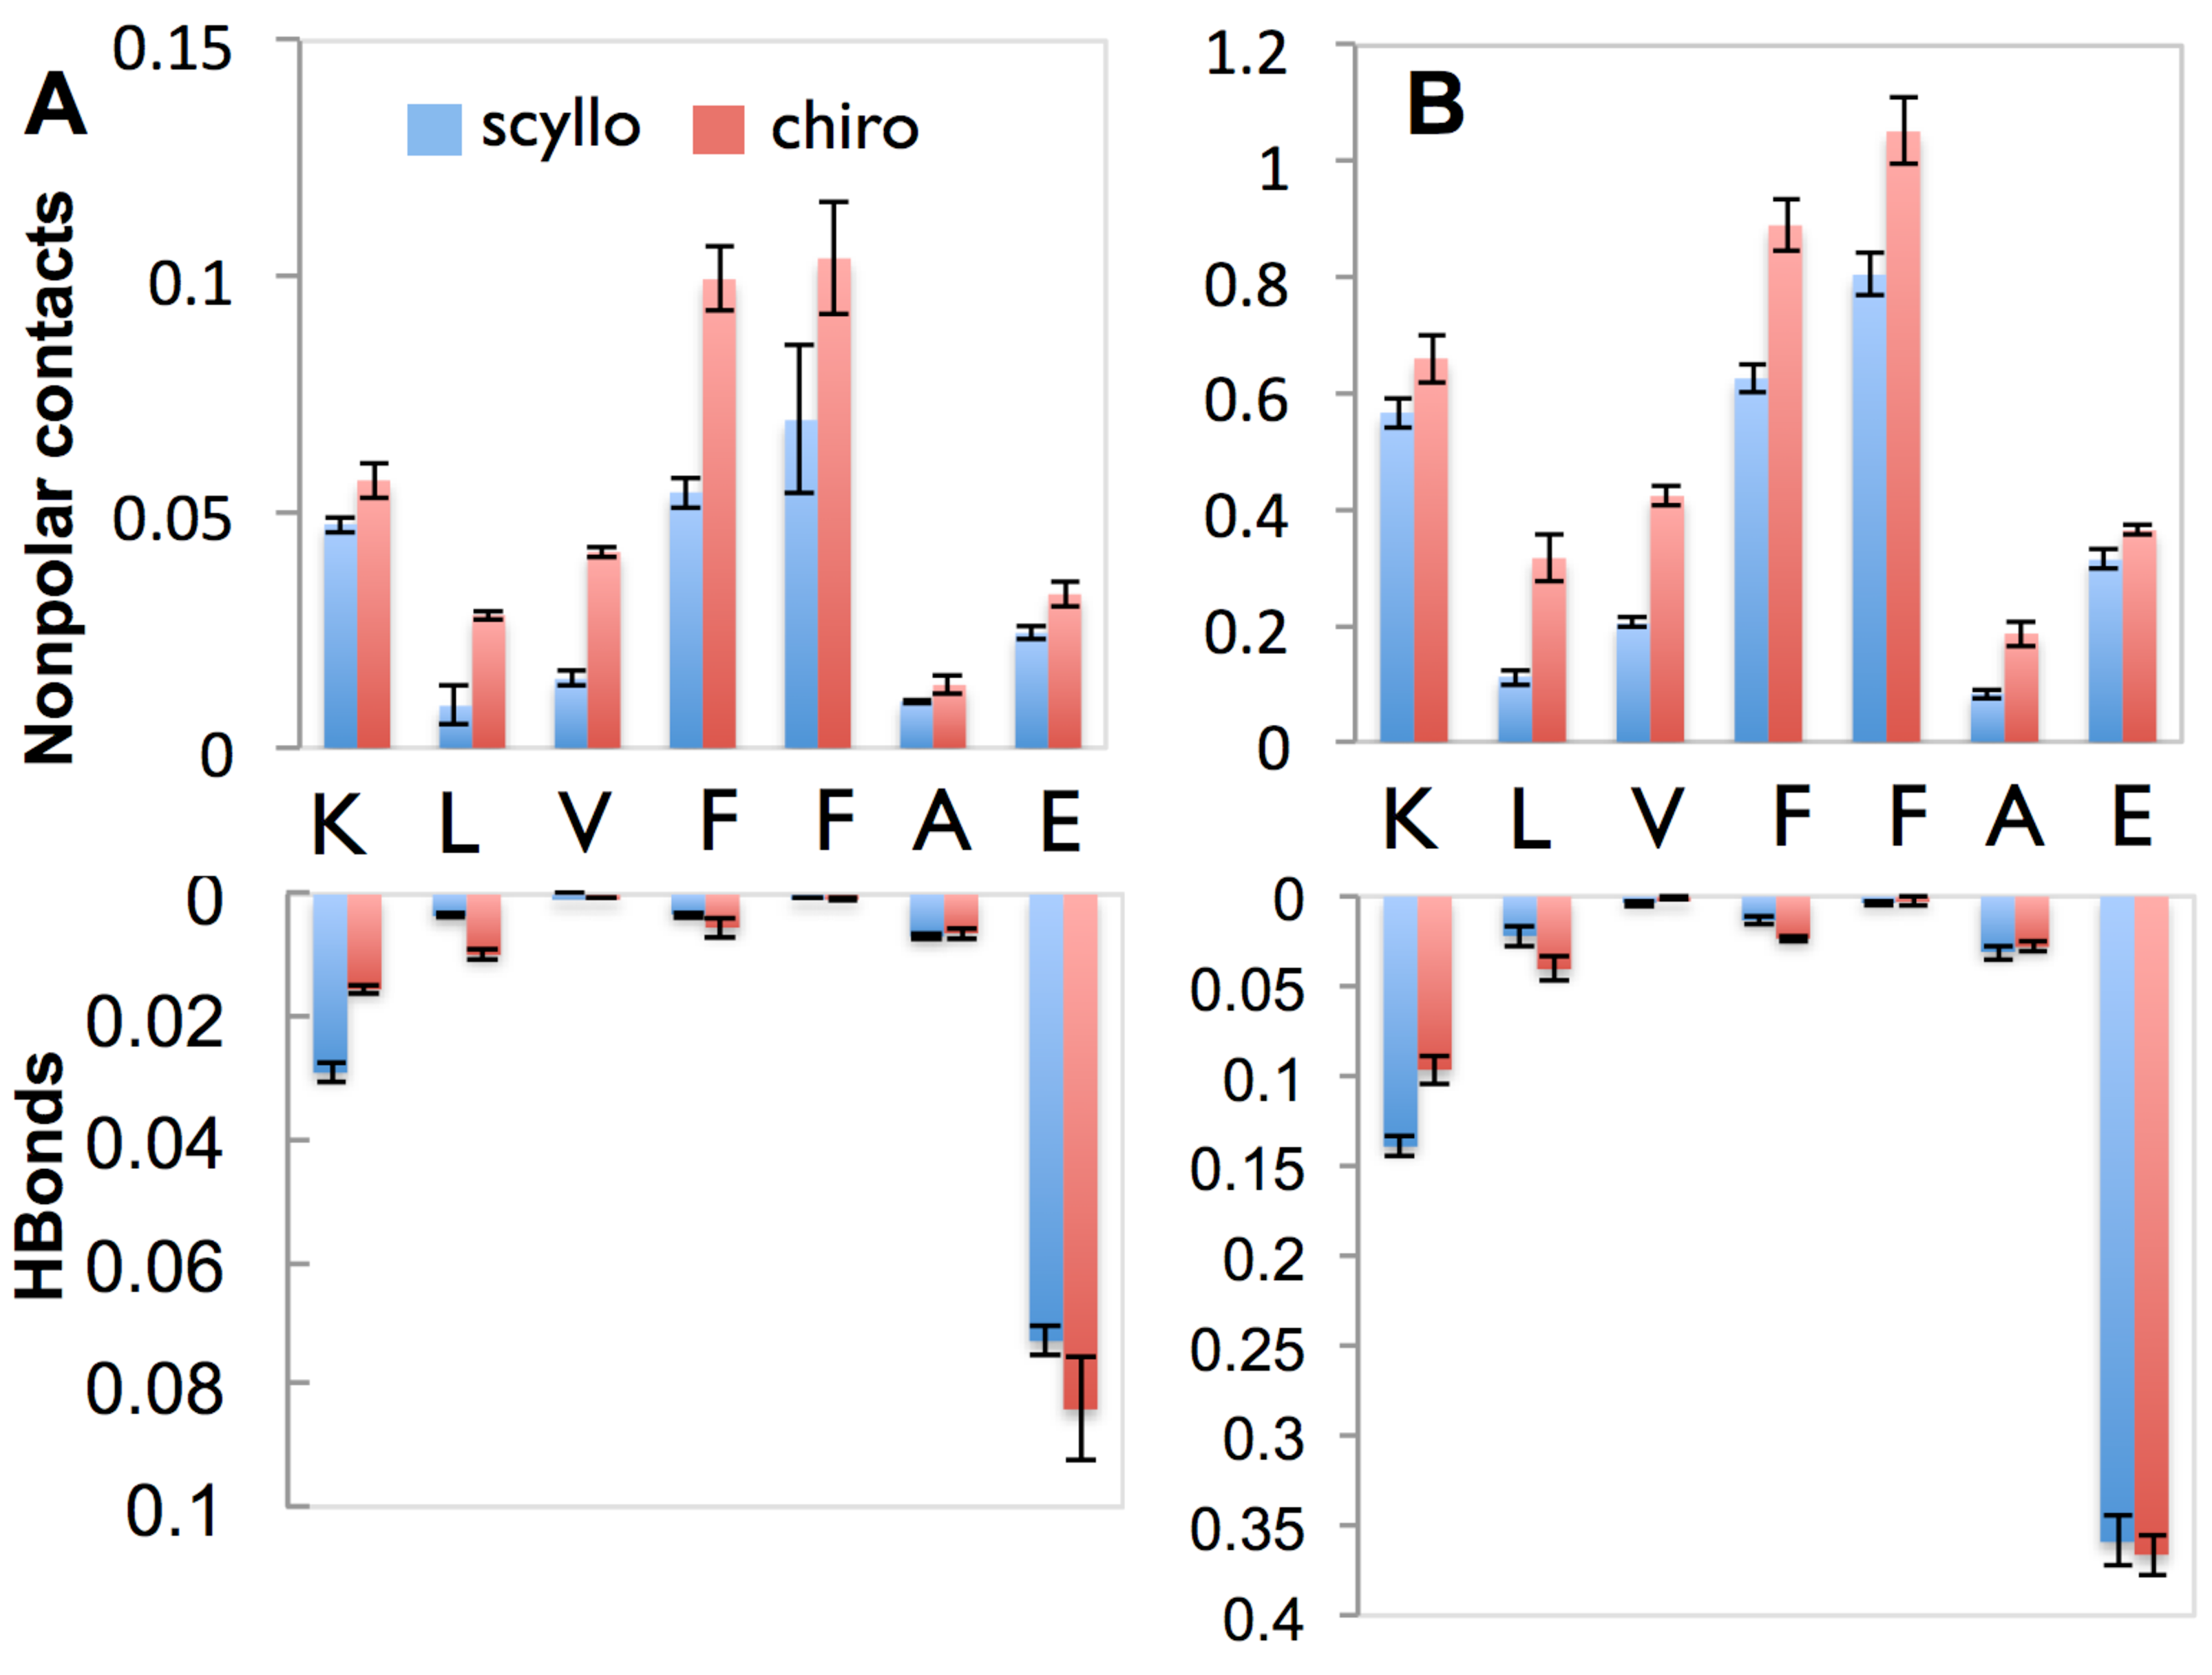
\includegraphics[width=15.15cm]{figures/appendixA/inos2_figures_SI_betaBinding.pdf}
\caption[Time-averaged number of hydrogen bonds and nonpolar made by inositol to each residue of the $\beta$-oligomer]{Time-averaged number of hydrogen bonds (top), and nonpolar (bottom) made by inositol to each residue of the $\beta$-oligomer at inositol:peptide molar ratios of (A) below 1:1, and (B) 64:16 (effective inositol concentration of 208 mM).}
\label{fig:SI-betaBinding}
\end{figure}